%%%%%%%%%%%%%%%%%%%%%%%%%%%%%%%%%%%%%%%%%%%%%%%%%%%%%%%
%                File: OpEx_style.tex                 %
%             Created: 2 September 2009               %
%                Updated: 15 May 2015                 %
%                                                     %
%           LaTeX template file for use with          %
%           OSA's journals Optics Express,            %
%             Biomedical Optics Express,              %
%            and Optical Materials Express            %
%                                                     %
%  send comments to Theresa Miller, tmiller@osa.org   %
%                                                     %
% This file requires style file, opex3.sty, under     %
	%              the LaTeX article class                %
%                                                     %
%   \documentclass[10pt,letterpaper]{article}         %
%   \usepackage{opex3}                                %
%                                                     %
%                                                     %
%       (c) 2015 Optical Society of America           %
%%%%%%%%%%%%%%%%%%%%%%%%%%%%%%%%%%%%%%%%%%%%%%%%%%%%%%%

%%%%%%%%%%%%%%%%%%%%%%% preamble %%%%%%%%%%%%%%%%%%%%%%%%%%%
\documentclass[10pt,letterpaper]{article}
\usepackage{opex3}
\usepackage{color}
\usepackage{threeparttable}
\usepackage{cite}
\usepackage{subfigure}
\usepackage{float}
\usepackage{amsmath}

%%%%%%%%%%%%%%%%%%%%%%% begin %%%%%%%%%%%%%%%%%%%%%%%%%%%%%%
\begin{document}

\title{Coherent control of high-order harmonic generation by a chirped few-cycle pulse in a two-level system with a permanent dipole moment}

\author{Pidong Hu,$^1$ Yueping Niu,$^{1,3}$ Shangqing Gong,$^{1,4}$  and Chengpu Liu$^{2,*}$}

\address{$^1$Department of Physics, East China University of Science and Technology, \\
Meilong Road 130, Shanghai 200237, China\\
$^2$State Key Laboratory of High Field Laser Physics, Shanghai Institute of Optics and Fine Mechanics, Chinese Academy of Sciences, Qinghe Road 390, Shanghai 201800, China\\
$^{3}$niuyp@ecust.edu.cn\\
$^{4}$sqgong@ecust.edu.cn
}

\email{*chpliu@siom.ac.cn}

% \homepage{http:...} %% author's URL, if desired

%%%%%%%%%%%%%%%%%%% abstract and OCIS codes %%%%%%%%%%%%%%%%
%% [use \begin{abstract*}...\end{abstract*} if exempt from copyright]

\begin{abstract}
The high-order harmonic generation in a two-level system with a permanent dipole moment is investigated, while a chirped few-cycle laser pulse is used to control the coherence of the harmonic spectrum. The situation that the laser pulse propagates in the medium is also considered. The harmonic spectrum can be obtained by numerically solving the nonlinear Bloch equations or the Maxwell-Bloch equations respectively for the non-propagation and propagation cases. The time-frequency characteristic of the harmonic spectrum is analyzed for the non-propagation case by means of the wavelet transform of induced time-dependent mean dipole moment. The cutoff harmonic can be dramatically extended due to the permanent dipole moment. Moreover, the coherence of a large range of harmonics in the plateau region can be enhanced due to the chirped frequency added into the laser pulse. By selecting several orders of the harmonics within the plateau, an attosecond pulse train with only two individual peaks can be generated with Fourier synthesis method. While, if the propagation effect is considered, an isolated attosecond pulse with considerable intensity can be generated by synthesizing the harmonics in the cutoff region for a proper propagation distance.
\end{abstract}

\ocis{(140.7090) Ultralfast lasers; (190.4180) Multiphoton processes; (320.7110) Ultrafast nonlinear optics; (190.5530) Pulse propagation and solitons.} % REPLACE WITH CORRECT OCIS CODES FOR YOUR ARTICLE, MINIMUM OF TWO; Avoid using the OCIS codes for “General” or “General science” whenever possible.
%For a complete list of OCIS codes, visit: http://www.opticsinfobase.org/submit/ocis/

%%%%%%%%%%%%%%%%%%%%%%% References %%%%%%%%%%%%%%%%%%%%%%%%%
%%%%%%%%%%%%%%%%%%%%%%% References %%%%%%%%%%%%%%%%%%%%%%%%%
\begin{thebibliography}{99}
\bibitem{Mokhtari-chemical-bond-Nature-1990}A. Mokhtari, P. Cong, J. L. Herek, and A. H. Zewail, ``Direct femtosecond mapping of trajectories in a chemical reaction," \nat {\bf 348}, 225--227 (1990).

\bibitem{Ergler-Vibration-PRL-2006}T. Ergler, B. Feuerstein, A. Rudenko, K. Zrost, C. D. Schröter, R. Moshammer, and J. Ullrich, ``Quantum-phase resolved mapping of ground-state vibrational ${\rm{D}}_{2}$ wave packets via selective depletion in intense laser pulses," \prl {\bf 97}, 103004 (2006).

\bibitem{Uiberacker-Attosecond-real-time-Nature-2007}M. Uiberacker, T. Uphues, M. Schultze, A. J. Verhoef, V. Yakovlev, M. F. Kling, J. Rauschenberger, N. M. Kabachnik, H. Schroder, M. Lezius, K. L. Kompa, H. G. Muller, M. J. J. Vrakking, S. Hendel, U. Kleineberg, U. Heinzmann, M. Drescher, and F. Krausz, ``Attosecond real-time observation of electron tunnelling in atoms," \nat {\bf 446}, 627--632 (2007).

\bibitem{Krausz-Attosecon-Review-2009}F. Krausz and M. Ivanov, ``Attosecond physics," \rmp {\bf 81}, 163--234 (2009).

\bibitem{Shore-HHG-Origin-JPB-1987}B. W. Shore and P. L. Knight, ``Enhancement of high optical harmonics by excess-photon ionisation," J. Phys. B: At. Mol. Opt. Phys. {\bf 20}, 413 (1987).

\bibitem{McPherson-Early-HHG-JOSAB-1987}A. McPherson, G. Gibson, H. Jara, U. Johann, T. S. Luk, I. A. McIntyre, K. Boyer, and C. K. Rhodes, ``Studies of multiphoton production of vacuum-ultraviolet radiation in the rare gases," \josab {\bf 4}, 595--601 (1987).

\bibitem{Ferray-Early-HHG-JPB-1988}M. Ferray, A. L'Huillier, X. F. Li, L. A. Lompre, G. Mainfray, and C. Manus, ``Multiple-harmonic conversion of 1064 nm radiation in rare gases," J. Phys. B: At. Mol. Opt. Phys. {\bf 21}, L31 (1988).

\bibitem{Corkum-PRL-1993}P. B. Corkum, ``Plasma perspective on strong field multiphoton ionization," \prl {\bf 71}, 1994--1997 (1993).

\bibitem{Lewenstein-SFA-PRA-1994}M. Lewenstein, P. Balcou, M. Y. Ivanov, A. L'Huillier, and P. B. Corkum, ``Theory of high-harmonic generation by low-frequency laser fields," \pra {\bf 49}, 2117--2132 (1994).

\bibitem{1997Review}M. Protopapas, C. H. Keitel, and P. L. Knight, ``Atomic physics with super-high intensity lasers," Rep. Prog. Phys. {\bf 60}, 389--486 (1997).

\bibitem{Sundaram-Early-Two-Level-PRA-1990}B. Sundaram and P. W. Milonni, ``High-order harmonic generation: simplified model and relevance of single-atom theories to experiment," \pra {\bf 41}, 6571--6573 (1990).

\bibitem{Ivanov-Early-Two-Level-PRA-1993}M. Y. Ivanov and P. B. Corkum, ``Generation of high-order harmonics from inertially confined molecular ions," \pra {\bf 48}, 580--590 (1993).

\bibitem{Kaplan-Early-Two-Level-PRA-1994}A. E. Kaplan and P. L. Shkolnikov, ``Superdressed two-level atom: very high harmonic generation and multiresonances," \pra {\bf 49}, 1275--1280 (1994).

\bibitem{Gauthey-Early-Two-Level-PRA-1997}F. I. Gauthey, B. M. Garraway, and P. L. Knight, ``High harmonic generation and periodic level crossings," \pra {\bf 56}, 3093--3096 (1997).

\bibitem{Faria-Two-Level-Three-Step-PRA-2002}C. Figueira de Morisson Faria and I. Rotter, ``High-order harmonic generation in a driven two-level atom: periodic level crossings and three-step processes," \pra {\bf 66}, 013402 (2002).

\bibitem{Sansone-Polarization-gate-Nature-2006}G. Sansone, E. Benedetti, F. Calegari, C. Vozzi, L. Avaldi, R. Flammini, L. Poletto, P. Villoresi, C. Altucci, R. Velotta, S. Stagira, S. De Silvestri, and M. Nisoli, ``Isolated single-cycle attosecond pulses," Science {\bf 314}, 443--446 (2006).

\bibitem{Carrera-Chirp-PRA-2007}J. J. Carrera and S.-I. Chu, ``Extension of high-order harmonic generation cutoff via coherent control of intense few-cycle chirped laser pulses," \pra {\bf 75}, 033807 (2007).

\bibitem{ZengZhinan-Two-Color-PRL-2007}Z. Zeng, Y. Cheng, X. Song, R. Li, and Z. Xu, ``Generation of an extreme ultraviolet supercontinuum in a two-color laser field," \prl {\bf 98}, 203901 (2007).

\bibitem{ChangZenghu-Combination-PRA-2007}Z. Chang, ``Controlling attosecond pulse generation with a double optical gating," \pra {\bf 76}, 051403 (2007).

\bibitem{Gong-Two-Level-Two-Color-JMO-1999}S. Gong, Z. Wang, S. Du, and Z. Xu, ``Coherent control of high-order harmonic generation in a two-level atom driven by intense two-colour laser fields," \jmo {\bf 46}, 1669--1676 (1999).

\bibitem{WANG-ZHONG-YANG-Two-Level-Attosecond-generation-1999}Z. Wang, S. Gong, and Z. Xu, ``Attosecond light pulse generation in a strongly driven two-level atom," Acta Phys. Sin. {\bf 48}, 961--965 (1999).

\bibitem{LiuChengpu-Two-Level-PRA-2004}C. Liu, S. Gong, R. Li, and Z. Xu, ``Coherent control in the generation of harmonics and hyper-Raman lines from a strongly driven two-level atom," \pra {\bf 69}, 023406 (2004).

\bibitem{YangWeifeng-Two-Level-PLA-2007}W. Yang, S. Gong, R. Li and Z. Xu, ``Generation of attosecond pulses in a system with permanent dipole moment," Phys. Lett. A {\bf 362}, 37--41 (2007).

\bibitem{CuiNi2010NJP-wavelet}N. Cui, Y. Xiang, Y. Niu, and S. Gong, ``Coherent control of terahertz harmonic generation by a chirped few-cycle pulse in a quantum well," New J. Phys. {\bf 12}, 013009 (2010).

\bibitem{2009Review}P. Sali\`{e}res and I. Christov, ``Macroscopic effects in high-order harmonic
generation," in \emph{Strong Field Laser Physics}, Thomas Brabec, ed. (Springer, 2009).

\bibitem{Kalosha-Two-Level-PRL-1999}V. P. Kalosha and J. Herrmann, ``Formation of optical subcycle pulses and full Maxwell-Bloch solitary waves by coherent propagation effects," \prl {\bf 83}, 544--547 (1999).

\bibitem{Ziolkowski-Two-Level-Method-PRA-1995}R. W. Ziolkowski, J. M. Arnold, and D. M. Gogny, ``Ultrafast pulse interactions with two-level atoms," \pra {\bf 52}, 3082--3094 (1995).


%\begin propagation references
\bibitem{Pan-Ruiqin-Permanent-dipole-moment-2011}R. Pan, ``Few-cycle ultrashort pulse laser propagation in organic molecular material," Acta Sinica Quantum Optica {\bf 17}, 52--57 (2011).

\bibitem{Xiao-Jian-PRA-2002}J. Xiao, Z. Wang, and Z. Xu, ``Area evolution of a few-cycle pulse laser in a two-level-atom medium," \pra {\bf 65}, 031402 (2002).

\bibitem{Xia-Keyu-OE-2005}K. Xia, S. Gong, C. Liu, X. Song, and Y. Niu, ``Near dipole-dipole effects on the propagation of few-cycle pulse in a dense two-level medium," \opex {\bf 13}, 5913--5924 (2005).

%\end propagation references

\bibitem{MyOE2013}P. Hu, Y. Niu, Y. Xiang, and S. Gong, ``Above-threshold ionization by few-cycle phase jump pulses," \opex {\bf 21}, 24309--24317 (2013).

\bibitem{TongXiaoMin2000PRA-Wavelet}X.-M. Tong and S.-I. Chu, ``Probing the spectral and temporal structures of high-order harmonic generation in intense laser pulses," \pra {\bf 61}, 021802(R) (2000).

\bibitem{Yee}K. S. Yee, ``Numerical solution of initial boundary value problems involing Maxwell's equations in isotropic media," \aprop {\bf 14}, 302--307 (1966).

\bibitem{Mur-Absorption}G. Mur, ``Absorbing boundary conditions for the finite-difference approximation of the time-domain electromagnetic-field equations," IEEE. Trans. Electronmagn. Compat. {\bf EMC-23}, 377--382 (1981).
	
\end{thebibliography}

%%%%%%%%%%%%%%%%%%%%%%%%%%  body  %%%%%%%%%%%%%%%%%%%%%%%%%%
\section{Introduction}
Femtosecond laser technology has obtained rapid development over the past decades, it provides us important experiment tools to study the strong-filed physics as well as the ultrafast phenomena. People can observe the ultra-fast dynamic chemical reaction process using the femtosecond technology, such as, the breaking and restructuring of the chemical bond \cite{Mokhtari-chemical-bond-Nature-1990} and the vibrations of an atom or a molecule \cite{Ergler-Vibration-PRL-2006}. However, if we want to explore the faster physics phenomena, including the electron transition and electron vibration, the sub-femtosecond or even the attosecond pulse should be used \cite{Uiberacker-Attosecond-real-time-Nature-2007}. In recent decades, one of the most important and effective method to generate attosecond laser pulse is the Fourier synthesis of the high-order harmonics. Krausz's team first obtained the sub-femtosecond pulse output (650 as) in experiment in 2003 \cite{Krausz-Attosecon-Review-2009}. From then on, this method gained extensive attention all over the world. Especially, Krausz's team obtained an 80 as pulse by utilizing a 3.3 fs driving laser pulse, which broke the limit of 100 as \cite{Krausz-Attosecon-Review-2009}.

High-order harmonic generation (HHG ) is first proposed by Shore and Knight in 1987 \cite{Shore-HHG-Origin-JPB-1987}, and subsequently, observed experimentally by McPherson \cite{McPherson-Early-HHG-JOSAB-1987} and Farray \cite{Ferray-Early-HHG-JPB-1988}. Its intuitive physical mechanism can be summarized as a \emph{three-step} model first proposed by Corkum \cite{Corkum-PRL-1993} and later developed by Lewenstein \emph{et al.} \cite{Lewenstein-SFA-PRA-1994}: first, electrons are liberated from the parent ion via tunneling ionization, then they move away and acquire energy from the laser field, finally small part of them may return back to the parent ion and recombine to the initial ground state with a harmonic photon emitted. The whole HHG spectrum has a unique character: the first few harmonics decay exponentially rapidly followed by a plateau in which the harmonic intensity varies weakly with order, and eventually an abrupt cut-off occurs \cite{1997Review}. In contrast, as for a two-level atomic system, if the driving laser field is not strong enough and electron hardly is ionized, and the laser center frequency is much less than the atomic transition frequency, a HHG process can also be demonstrated and the corresponding HHG spectrum also process a long generic plateau and  clear cutoff \cite{Sundaram-Early-Two-Level-PRA-1990,Ivanov-Early-Two-Level-PRA-1993,Kaplan-Early-Two-Level-PRA-1994,Gauthey-Early-Two-Level-PRA-1997}. This kind of HHG has no connection with the so-called \emph{three-step} model. The origin of the plateau is clarified by Gauthey \emph{et al.} \cite{Gauthey-Early-Two-Level-PRA-1997} as is linked to the rapid level crossing at each half-cycle of the laser period and the cutoff position analytically presented under a driven two-level model is in a good agreement with the numerical simulation result. Later, Faria \emph{et al.} \cite{Faria-Two-Level-Three-Step-PRA-2002} extended this two-level model with an analogous \emph{three-step} model to explain the harmonic generation process: a population transfer occurs from the field-dressed adiabatic lower state to the upper state at the time for level crossing, then the system acquires energy from the laser field, finally decays back to the lower state and radiates a harmonic photon with the energy equaling to the transient transition separation.

Fourier transformation to the harmonics within the plateau or the cut-off part of the spectra referring filtering or other technology is a routine tool to make an attosecond pulse train (APT) or isolated attosecond pulse (IAP) generated. Since the HHG spectra is sensitive to the driving pulse, quantum control schemes for high quality IAP or APT obtaining have been demonstrated widely, such as polarization gating \cite{Corkum-PRL-1993,Sansone-Polarization-gate-Nature-2006}, nonlinear chirped laser pulse \cite{Carrera-Chirp-PRA-2007}, two-color laser pulse \cite{ZengZhinan-Two-Color-PRL-2007}, and some kind of combination of these methods \cite{ChangZenghu-Combination-PRA-2007}, etc.. In the driven two-level regime, the two-color laser pulse \cite{Gong-Two-Level-Two-Color-JMO-1999,WANG-ZHONG-YANG-Two-Level-Attosecond-generation-1999,LiuChengpu-Two-Level-PRA-2004} has been demonstrated, and it is found that the plateau can be extended. The polar molecule system with a permanent dipole moment demonstrated that the existence of the permanent dipole moment can significantly extend the spectrum plateau (even to X-ray range) \cite{YangWeifeng-Two-Level-PLA-2007}. Moreover, if a hyperbolic tangent chirped few-cycle laser pulse is used to drive a two-level quantum well, an ultra-broad super-continuum can be obtained and can be used to synthesize an isolated terahertz pulse \cite{CuiNi2010NJP-wavelet}. Therefore, this paper proposes that one can control the matter and the driving laser pulse at the same time. The plateau extension is expected with the help of permanent dipole moment, meanwhile, coherent enhancement for the HHG spectrum is expected by modulating the laser pulse with a chirp.

Actually, almost all the studies about HHG based on the driven two-level model just considered the single-particle-response, namely, the two-level system is only one atom, one molecule or one quantum well, etc. However, there are thousands of particles and the laser pulse and generated harmonic will propagate through the medium in the real experiment. As we know, in the ionization regime, if the driving pulse and the harmonic have the same phase velocity as they travel through the medium, the harmonic signal will achieve significant increase \cite{2009Review}. Many studies based on the driven two-level model with dense medium also have been done \cite{Kalosha-Two-Level-PRL-1999,Xiao-Jian-PRA-2002,Xia-Keyu-OE-2005,Pan-Ruiqin-Permanent-dipole-moment-2011,Ziolkowski-Two-Level-Method-PRA-1995}, however, their focus is mainly concentrated on the modulation of the laser pulse during the propagation process. Therefore, the macroscopic propagation process will be investigated in this paper and is expected to enhance the harmonic signal.

\section{Theoretical models and methods}
For the two cases of propagation considered or not, both the simulation model and the numerical solving method are different. In simple terms, non-propagation case need to solve the nonlinear Bloch equations with Runge-Kutta method and the other case need to solve the Maxwell-Bloch equations with finite-difference time-domain (FDTD) method. The two models and their corresponding solving methods will be separately introduced.

For the simple non-propagation case. Consider a two-level system where $\left| {\rm{1}} \right\rangle$ and $\left| {\rm{2}} \right\rangle$ represent the ground and excited states with the energy separation $ \omega_0 $ [Atomic units (a.u.) are used, unless otherwise mentioned]. Within this picture, the time-dependent wave function is

\begin{equation}
\left| {\varPsi \left( t \right)} \right\rangle  = {c_1}(t)\left| 1 \right\rangle  + {c_2}(t)\left| 2 \right\rangle,
\label{eq1}
\end{equation}
where $ c_{\rm{i}}(t) = \left\langle {\rm{i}} | \varPsi \left( t \right) \right\rangle(\rm{i}=1,2) $ denotes the overlap of the total wave function with the $\rm{i}^{th}$ state.

A semi-classical model is adopted in which the quantum system interacts with the classical laser field. The total Hamiltonian describing the interaction of the field with the two-level system which has permanent dipole moments is given by \cite{YangWeifeng-Two-Level-PLA-2007}

\begin{equation}
H = {H_0} + V = \left( {\begin{array}{*{20}{c}}
	{{E_1}}&0\\
	0&{{E_2}}
	\end{array}} \right) - E(t)\left( {\begin{array}{*{20}{c}}
	{{\mu _{11}}}&{{\mu _{12}}}\\
	{{\mu _{21}}}&{{\mu _{22}}}
	\end{array}} \right),
\label{eq2}
\end{equation}
where $ \mu_{\rm{ij}} $ are the dipole moment matrix elements, and ${E_1} =  - {1 \over 2}{\omega _0}$, ${E_2} =   {1 \over 2}{\omega _0}$. The linearly polarized Gaussian pulse is used to drive the system and the laser field is given by expression of

\begin{equation}
E(t) = {E_0}\exp \left[ { - 4\ln 2{{\left( {t/\tau } \right)}^2}} \right]\cos \left[ {{\omega _L}t + \varphi \left( t \right)} \right],
\label{eq3}
\end{equation}
where $ E_{0} $ is the field amplitude, $ \tau $ is the duration (full width at half maximum, FWHM), $ \omega_{\rm{L}} $ is the field angular frequency, and $ \varphi(t) $ is the time-dependent carrier envelope phase.

Finally, the following nonlinear Bloch equations can describe the system dynamics:

\begin{equation}
 {\partial _t}{u}\left( {t} \right) = {\omega _0}{v}\left( t \right) + 2\xi \Omega \left( t \right){v}\left( t \right),
\label{eq4}
\end{equation}
\begin{equation}
{\partial _t}{v}\left( {t} \right) =  - {\omega _0}{u}\left( t \right) + 2\Omega \left( t \right){w}\left( t \right) - 2\xi \Omega \left( t \right){u}\left( t \right),
\label{eq5}
\end{equation}
\begin{equation}
{\partial _t}{w}\left( {t} \right) =  - 2\Omega \left( t \right){v}\left( t \right).
\label{eq6}
\end{equation}
Where, $ u(t) $ and $ v(t) $ are the mean real and imaginary parts of polarization, respectively, $ w(t) $ is the mean population difference. $\Omega\left( t \right) = - \vec{\mu}_{21}\vec{E}\left(t\right)=\Omega_{0}/E_{0}\cdot E\left(t\right)$ is the Rabi frequency of the incident laser field with peak value of ${\Omega _0} =  - {\mu _{21}}{E_0}$, $\xi  = {{\left( {{\mu _{22}} - {\mu _{11}}} \right)} \mathord{\left/{\vphantom {{\left( {{\mu _{22}} - {\mu _{11}}} \right)} {2{\mu _{21}}}}} \right.\kern-\nulldelimiterspace} {2{\mu _{21}}}}$ is a dimensionless parameter which characterizes the permanent dipole moment. In the two-level model, the main observable of interest is $u(t)$, which leads to the coherent part of the light spectrum by Fourier transformation

\begin{equation}
P(\omega)= \left| \textrm{d}t\exp(i\omega t)\bar{N}u(t)\right|^2.
\label{eq7}
\end{equation}
Where $ \bar{N} $ is density of the medium, it is introduced here for the consistency with propagation situation discussed later. It is chosen as $ \bar{N}=7.5\times10^{24} \textrm{m}^{-3}$ for both the propagation and non-propagation cases. The system of evolution Eqs. (\ref{eq4})--(\ref{eq6}) can be solved numerically without making rotating-wave approximation by means of a fourth-order Runge-Kutta method. The Fourier transformation is performed using the Fast Fourier transformation algorithm.

Moreover, the time-frequency analysis is performed to the high-order harmonic generation by using the wavelet transform to the induced dipole moment ${u}\left( t \right)$ in order to investigate the temporal structures of HHG,

\begin{equation}
{A_\omega }\left( {t,\omega } \right) = \int {\bar{N}{u}\left( {t'} \right)} \sqrt \omega  {W}\left[ {\omega \left( {t - t'} \right)} \right]{\rm{d}}t',
\label{eq8}
\end{equation}
where  $ {W}(x) $ is the window function (also called the mother wavelet function) which is given here by the form of Morlet wavelet \cite{CuiNi2010NJP-wavelet,MyOE2013,TongXiaoMin2000PRA-Wavelet}

\begin{equation}
{{W}}\left( x \right) = \sqrt {\frac{{\rm{1}}}{{{\tau _{wav}}}}} {e^{ix}}{e^{ - {x^2}/2\tau _{wav}^2}},
\label{eq9}
\end{equation}
$ t $ and $ \omega $ denote the time and harmonic frequency at which the window function is centered. The envelope width $ \tau_{\rm{wav}} $ of the wavelet is set to 6.0 in our calculations.

As for the propagation process, the Maxwell-Bloch equations should be numerically solved. Now, propagation of a linearly polarized short laser pulse along the $ z $ axis to an input interface of the two-level medium at $ z=L_{1} $ is considered. Initially the pulse propagates in the vacuum of free space, then it penetrates into the medium with some reflects, the penetrating part propagates through the medium and finally exits again into the vacuum through the output interface at $ z=L_{2} $ \cite{Kalosha-Two-Level-PRL-1999}. If the laser field is assumed to polarize along  the $ x $ axis, then the Maxwell equations would take the form of

\begin{equation}
\begin{array}{l}
\smallskip
{\partial _t}{H_y}\left( {z,t} \right) =  - \frac{1}{{{\mu _0}}}{\partial _z}{E_x}\left( {z,t} \right)\;,\\
\smallskip
{\partial _t}{E_x}\left( {z,t} \right) =  - \frac{1}{{{\varepsilon _0}}}{\partial _z}{H_y}\left( {z,t} \right) - \frac{1}{{{\varepsilon _0}}}{\partial _t}{P_x}\left( {z,t} \right)\;,\\
\smallskip
{\partial _t}u\left( {z,t} \right) = {\omega _0}v\left( {z,t} \right) + 2\xi \Omega \left( {z,t} \right)v\left( {z,t} \right) - {{u\left( {z,t} \right)} \mathord{\left/
		{\vphantom {{u\left( {z,t} \right)} {{T_2}}}} \right.
		\kern-\nulldelimiterspace} {{T_2}}},\\
\smallskip
{\partial _t}v\left( {z,t} \right) =  - {\omega _0}u\left( {z,t} \right) + 2\Omega \left( {z,t} \right)w\left( {z,t} \right) - 2\xi \Omega \left( {z,t} \right)u\left( {z,t} \right) - {{v\left( {z,t} \right)} \mathord{\left/
		{\vphantom {{v\left( {z,t} \right)} {{T_2}}}} \right.
		\kern-\nulldelimiterspace} {{T_2}}},\\
\smallskip
{\partial _t}w\left( {z,t} \right) =  - 2\Omega \left( {z,t} \right)v\left( {z,t} \right) - {{\left[ {w\left( {z,t} \right) - {w_{0}}} \right]} \mathord{\left/
		{\vphantom {{\left[ {w\left( {z,t} \right) - {w_{0}}} \right]} {{T_1}}}} \right.
		\kern-\nulldelimiterspace} {{T_1}}}.
\end{array}
\label{eq10}
\end{equation}

Here $ E_{\rm{x}} $, $ H_{\rm{y}} $ is the laser pulse electric and magnetic field, respectively. $\mu_{0}$ and $ \epsilon_{0} $ are the vacuum permeability and vacuum permittivity, respectively. $w_0$ is the initial population difference. Maxwell equations are united with the Bloch equations here, and the physical quantities are not only dependent on the time but also dependent on the propagation distance, $ z $. Here the relaxation time of the two-level medium is considered, where $T_{1}$ is the excited-state lifetime and $T_{2}$ is the dephasing time. It is noted that, for the non-propagation case, the relaxation time are not considered because of that they are much longer than the laser-matter interaction time. $ P_{\rm{x}} $ is the macroscopic nonlinear polarization, and is given for two-level system as expression of \cite{Pan-Ruiqin-Permanent-dipole-moment-2011}

\begin{equation}
\begin{array}{l}
{P_x} =   \bar{N}tr\left( {\mathord{\buildrel{\lower3pt\hbox{$\scriptscriptstyle\rightharpoonup$}}
		\over \mu } \rho } \right)\\
\;\;\;\;\: =   \bar{N}\left( {{\mu _{11}}{\rho _{11}} + {\mu _{22}}{\rho _{22}} + {\mu _{12}}{\rho _{12}} + {\mu _{21}}{\rho _{21}}} \right)
\end{array}
\label{eq11}
\end{equation}
where $ \bar{N} $ is the density of the medium, ${\rho _{\rm{ij}}}\left( {\rm{i,j} = 1, 2} \right)$  is the density matrix element for the two-level system. If the system is closed (i.e., the system has no energy exchange with the outside environment),  $ P_{\rm{x}} $ can be expressed as

\begin{equation}
{P_x} =   \bar{N}{\mu _{21}}u + \bar{N}\xi {\mu _{21}}w + {{\bar{N}\left( {{\mu _{11}} + {\mu _{22}}} \right)} \mathord{\left/
		{\vphantom {{N\left( {{\mu _{11}} + {\mu _{22}}} \right)} 2}} \right.
		\kern-\nulldelimiterspace} 2}.
\label{eq12}
\end{equation}

Eq. (\ref{eq10}) can be solved using Yee's leap-frog FDTD discretization scheme \cite{Yee} with the iterative predictor-corrector method \cite{Ziolkowski-Two-Level-Method-PRA-1995}. Mur absorbing boundary conditions \cite{Mur-Absorption} were incorporated with FDTD discretization which can avoid the unphysical reflection from the finite calculation boundaries. Here, the initial pulse condition is given as

\begin{equation}
\begin{array}{l}
{E_x}\left( {z,t = 0} \right) = {E_0}\exp \left[ { - 4\ln 2{{\left( {\frac{{z - {z_0}}}{{c\tau }}} \right)}^2}} \right]\cos \left[ {{\omega _L}{{\left( {z - {z_0}} \right)} \mathord{\left/
			{\vphantom {{\left( {z - {z_0}} \right)} c}} \right.
			\kern-\nulldelimiterspace} c}} \right],\\
{H_y}\left( {z,t = 0} \right) = \sqrt {{{{\varepsilon _0}} \mathord{\left/
			{\vphantom {{{\varepsilon _0}} {{\mu _0}}}} \right.
			\kern-\nulldelimiterspace} {{\mu _0}}}} {E_x}\left( {z,t = 0} \right),
\end{array}
\label{eq13}
\end{equation}
where $ c $ is the light velocity in the vacuum. The choice of $ z_{0} $ can ensure that the pulse penetrates negligibly into the medium at $ t=0 $. In our calculations $ z_{0} $ is set to be $15\;\mu$m.

\section{Results and discussions}
First, the non-propagation case is discussed, as is generally done \cite{CuiNi2010NJP-wavelet,Faria-Two-Level-Three-Step-PRA-2002,Gauthey-Early-Two-Level-PRA-1997,Gong-Two-Level-Two-Color-JMO-1999,Kaplan-Early-Two-Level-PRA-1994,LiuChengpu-Two-Level-PRA-2004,YangWeifeng-Two-Level-PLA-2007,ZengZhinan-Two-Color-PRL-2007,WANG-ZHONG-YANG-Two-Level-Attosecond-generation-1999}. The two-level system with an energy separation $\omega_0=0.30\;\textrm{a.u.}$ is assumed initially in its ground state, then $ u(0)=v(0)=0 $ , and $ w(0)=-1 $. In addition, the dipole moment matrix element is $\mu_{21}=1.18\;\textrm{a.u.}$ (corresponds to $1.0\times10^{-29}\textrm{Asm}$) and no permanent dipole moment exists for the present. As for the driving laser pulse, its center frequency $ \omega_{\rm{L}}=0.056\;\rm{a.u.}$ corresponding to a wavelength of 814 nm, its duration $\tau=2T$ (about $ 5.43\;\rm{fs} $, $T$ is the laser period) and its peak Rabi frequency $ \Omega_{0}=0.30\;\rm{a.u.} $.

\begin{figure}[!htbp]
	\centering
	\subfigure{
		\label{fig1a}
		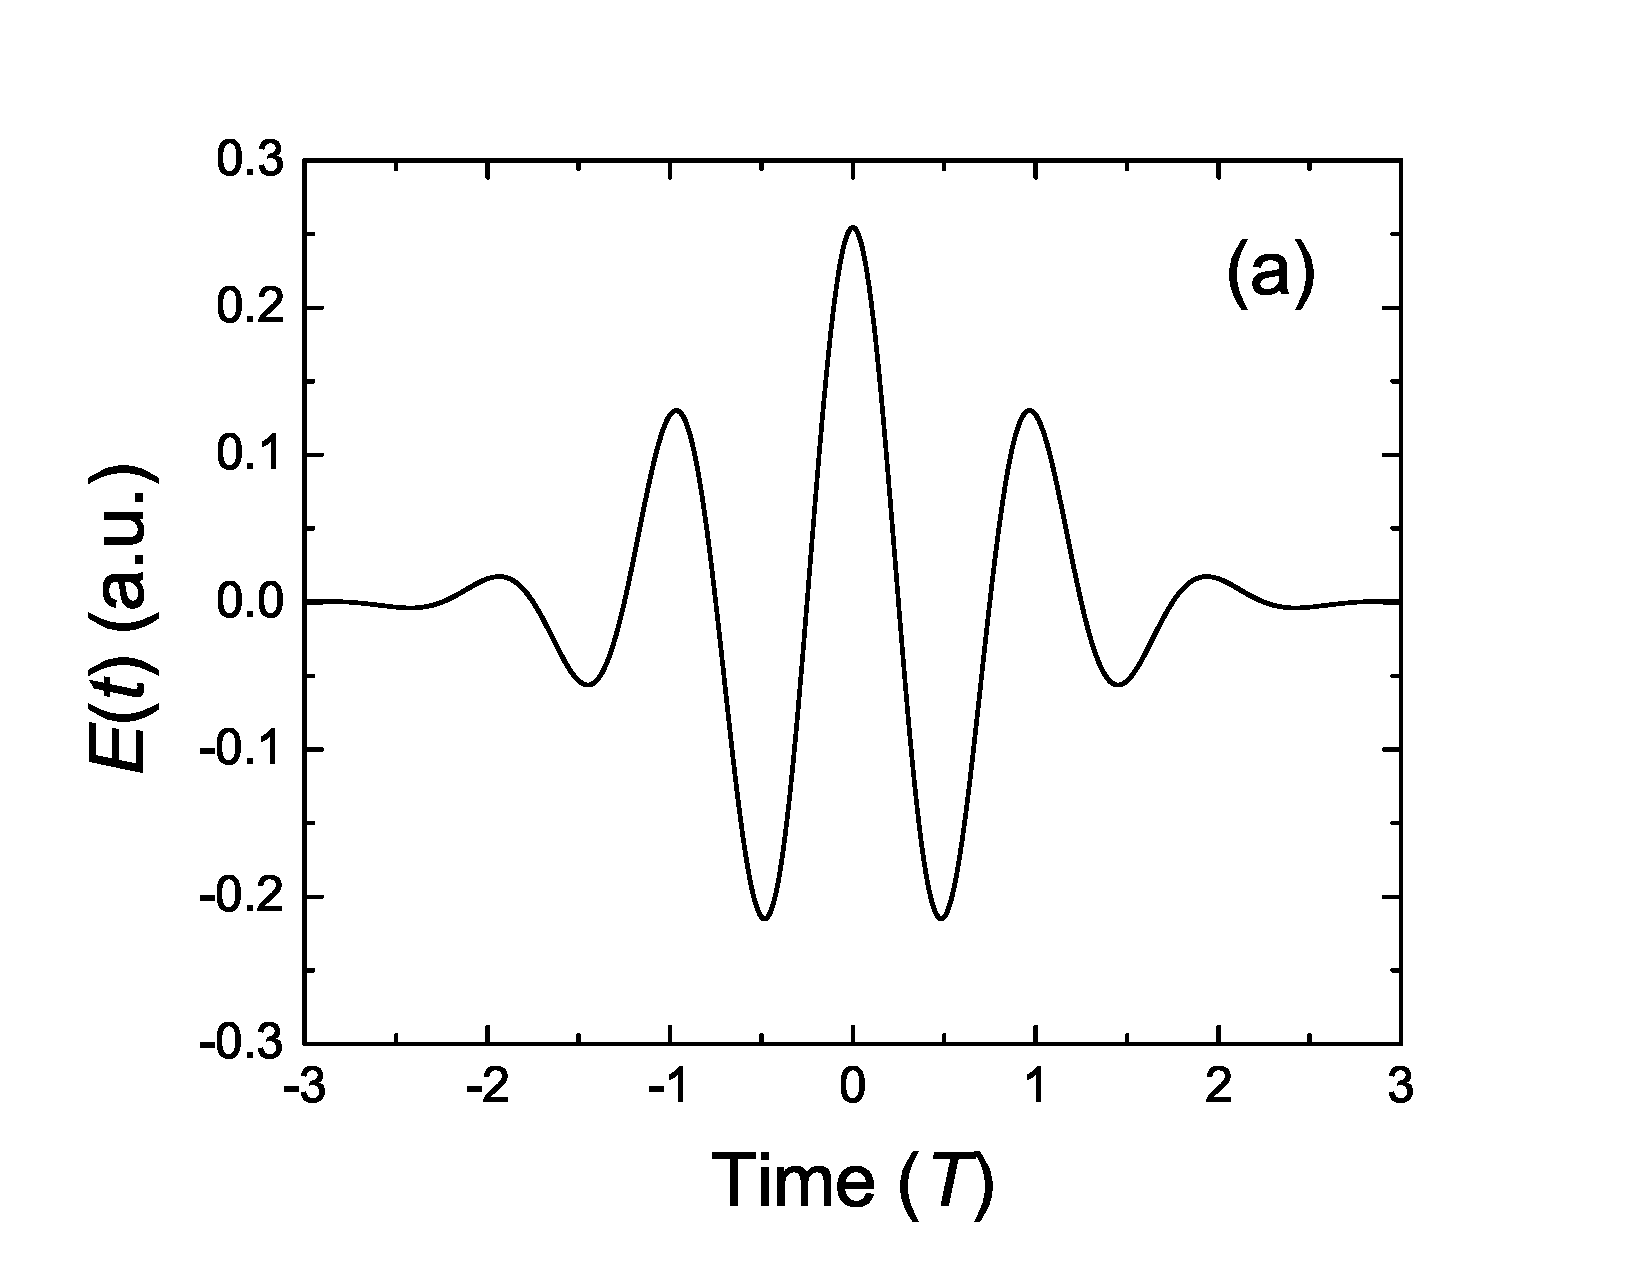
\includegraphics[width=0.4\textwidth]{fig1a.eps}
	}
	\subfigure{
		\label{fig1b}
		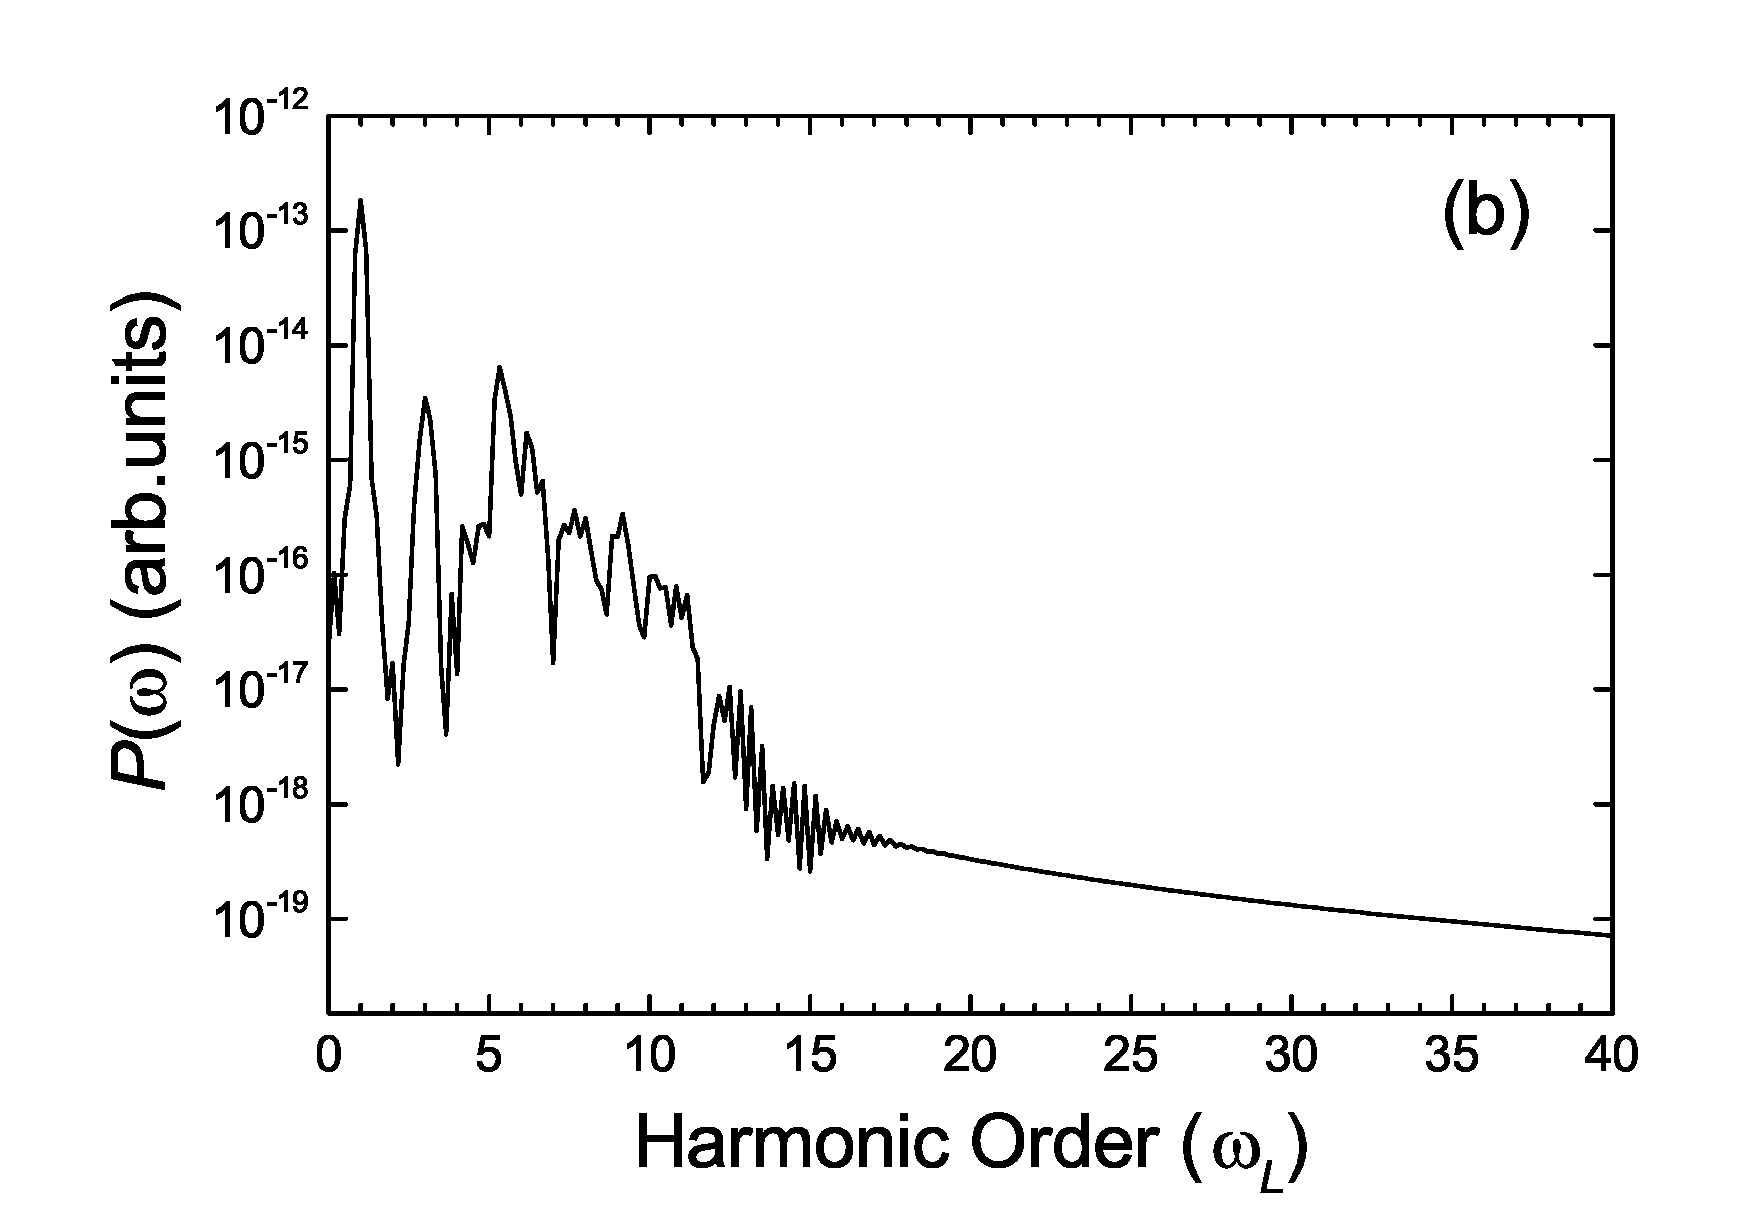
\includegraphics[width=0.42\textwidth]{fig1b.eps}
	}
	\caption{(a) Non-chirped Gaussian laser pulse, and (b) the corresponding HHG spectrum in the case of without a permanent dipole moment. Parameters for this laser pulse are set as: central frequency $\omega_L=0.056\;\textrm{a.u.}$, duration $\tau=5.43\;\rm{fs}$, and peak Rabi frequency $\Omega_0=0.30\;\textrm{a.u.}$.}
	\label{fig1}
\end{figure}

It has been well clarified that, as for a two-level atomic system, the occurrence of HHG is attributed to the rapid level crossing mechanism between the two field-dressed adiabatic states  \cite{Gauthey-Early-Two-Level-PRA-1997}. In the adiabatic basis, the Hamiltonian is diagonalized via a unitary transformation as,

\begin{equation}
\tilde H = \hat UH{\hat U^\dag } = \left( {\begin{array}{*{20}{c}}
	{{\varepsilon _ - }}&0\\
	0&{{\varepsilon _ + }}
	\end{array}} \right).
\label{eq14}
\end{equation}
with the field-dressed level energies \cite{YangWeifeng-Two-Level-PLA-2007}

\begin{equation}
{\varepsilon _ \pm } = \frac{1}{2}\left( { - \frac{{{\mu _{11}} + {\mu _{22}}}}{{{\mu _{21}}}}\Omega \left( t \right) \pm \sqrt {{{\left[ {2\xi \Omega \left( t \right) - {\omega _0}} \right]}^2} + {{\left[ {2\Omega \left( t \right)} \right]}^2}} } \right).
\label{eq15}
\end{equation}
and the frequency of harmonic emitted at time $t$ is determined by the energy separation of these two states at the same time,
\begin{equation}
\omega  = {\varepsilon _ + } - {\varepsilon _ - } = \sqrt {{{\left[ {2\xi \Omega \left( t \right) - {\omega _0}} \right]}^2} + {{\left[ {2\Omega \left( t \right)} \right]}^2}}  = N{\omega _L}.
\label{eq16}
\end{equation}
Where, $N$ is the harmonic order. Formula (\ref{eq16}) indicates clearly that the harmonic frequency varies over time and would have a maximum value $\omega_{\textrm{max}}$ with a cutoff order $N_{\textrm{max}}$ at time $t_{\textrm{max}}$ which can be found with the help of the $\omega-t$ plotting curve.
\begin{figure}[h]
	\centering
	\subfigure{
		\label{fig2a}
		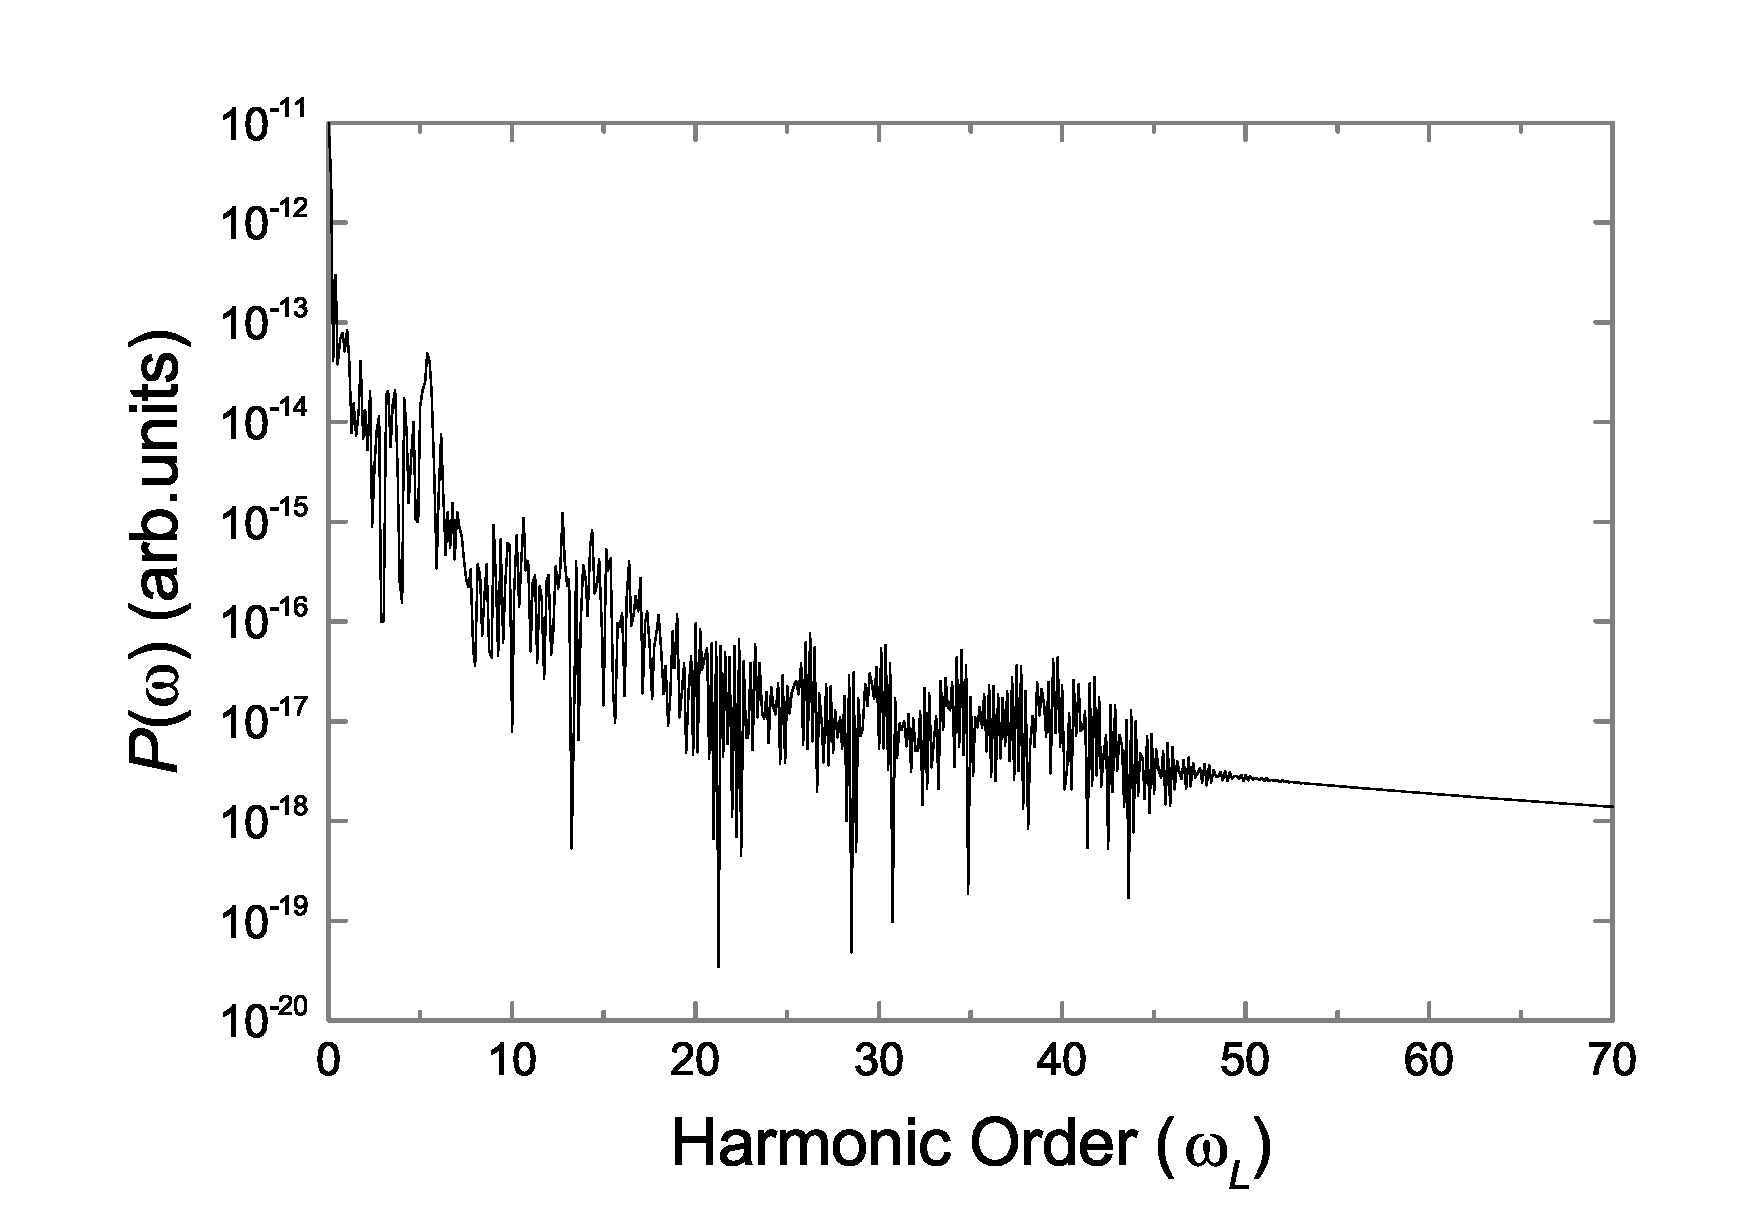
\includegraphics[width=0.42\textwidth,height=0.3\textwidth]{fig2a.eps}
	}
	\hspace{-0.1in}
	\subfigure{
		\label{fig2b}
		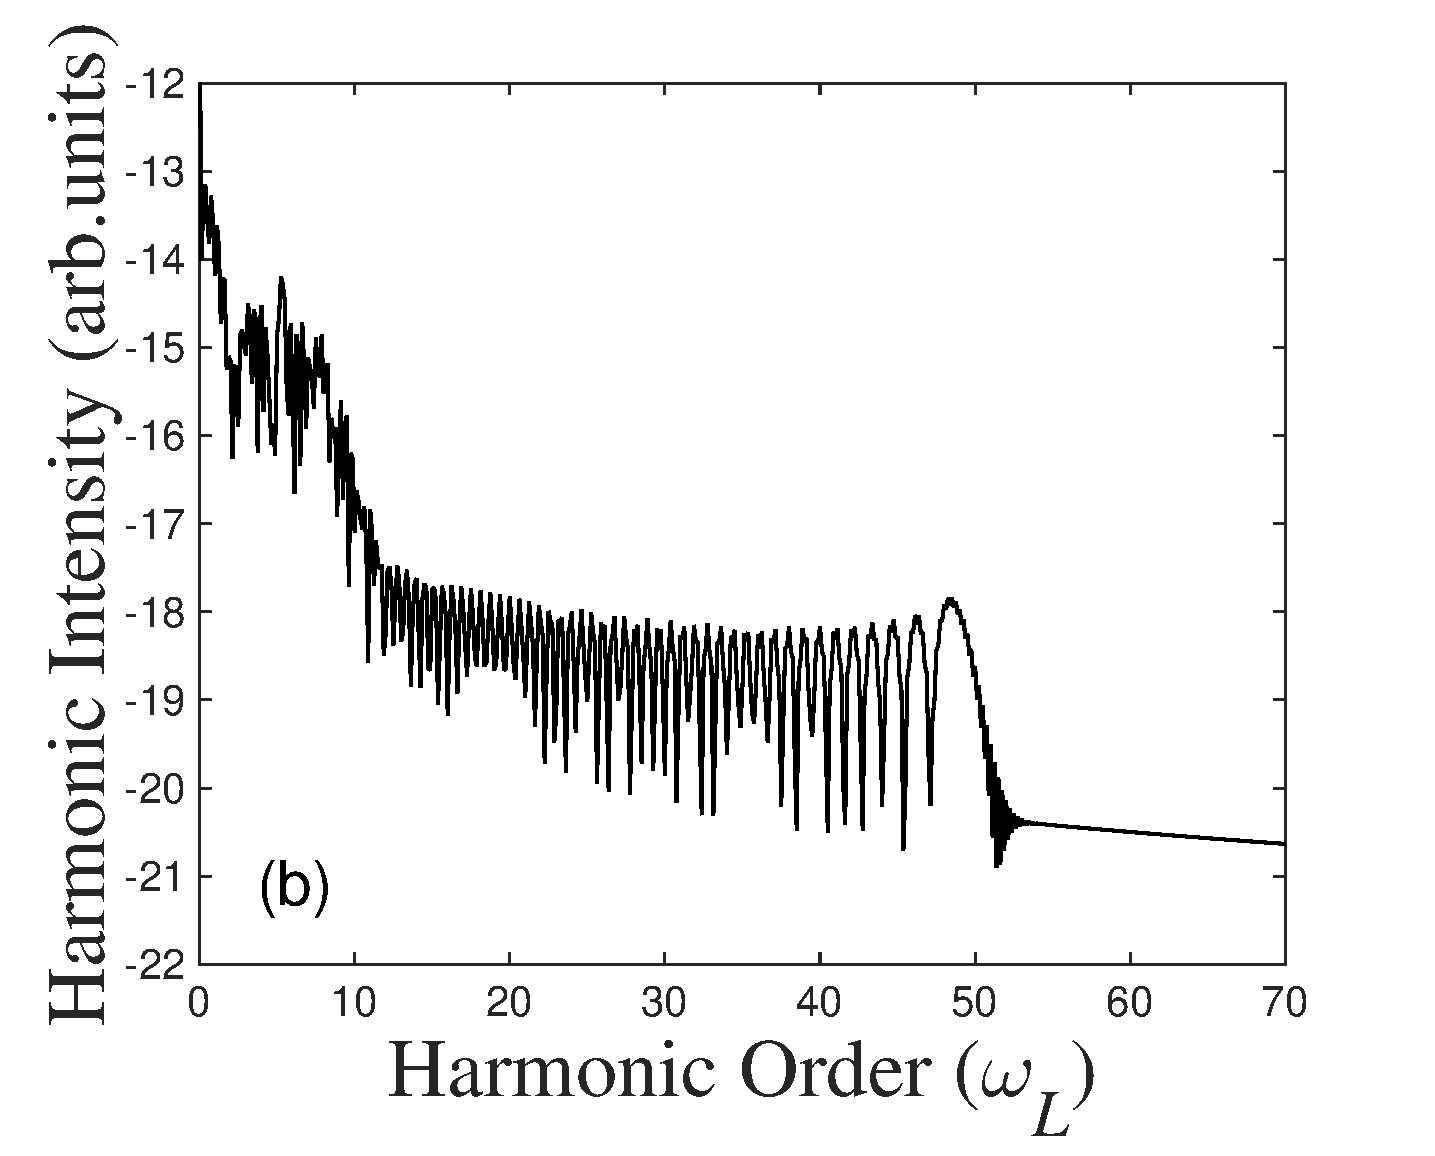
\includegraphics[width=0.42\textwidth,height=0.3\textwidth]{fig2b.eps}
	}
	
	\subfigure{
		\label{fig2c}
		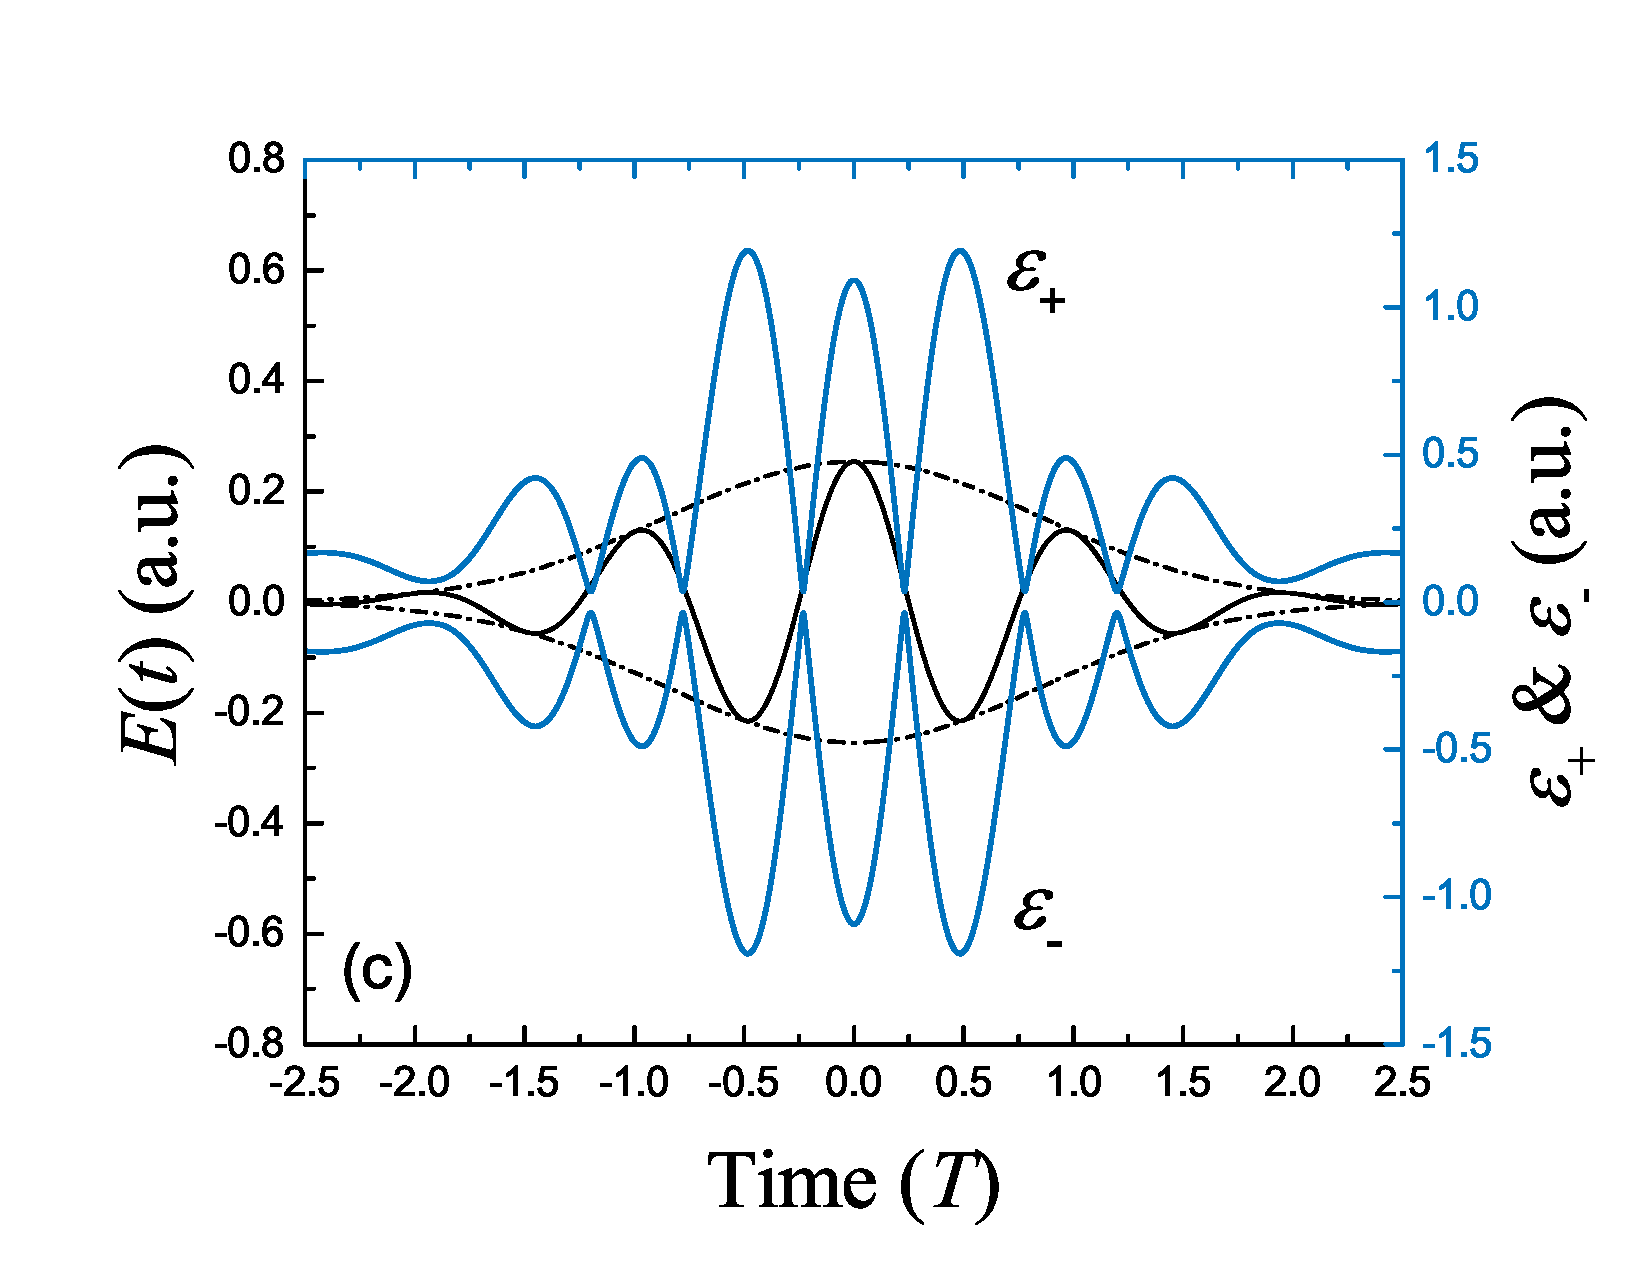
\includegraphics[width=0.45\textwidth,height=0.3\textwidth]{fig2c.eps}
	}
	\hspace{-0.25in}
	\subfigure{
		\label{fig2d}
		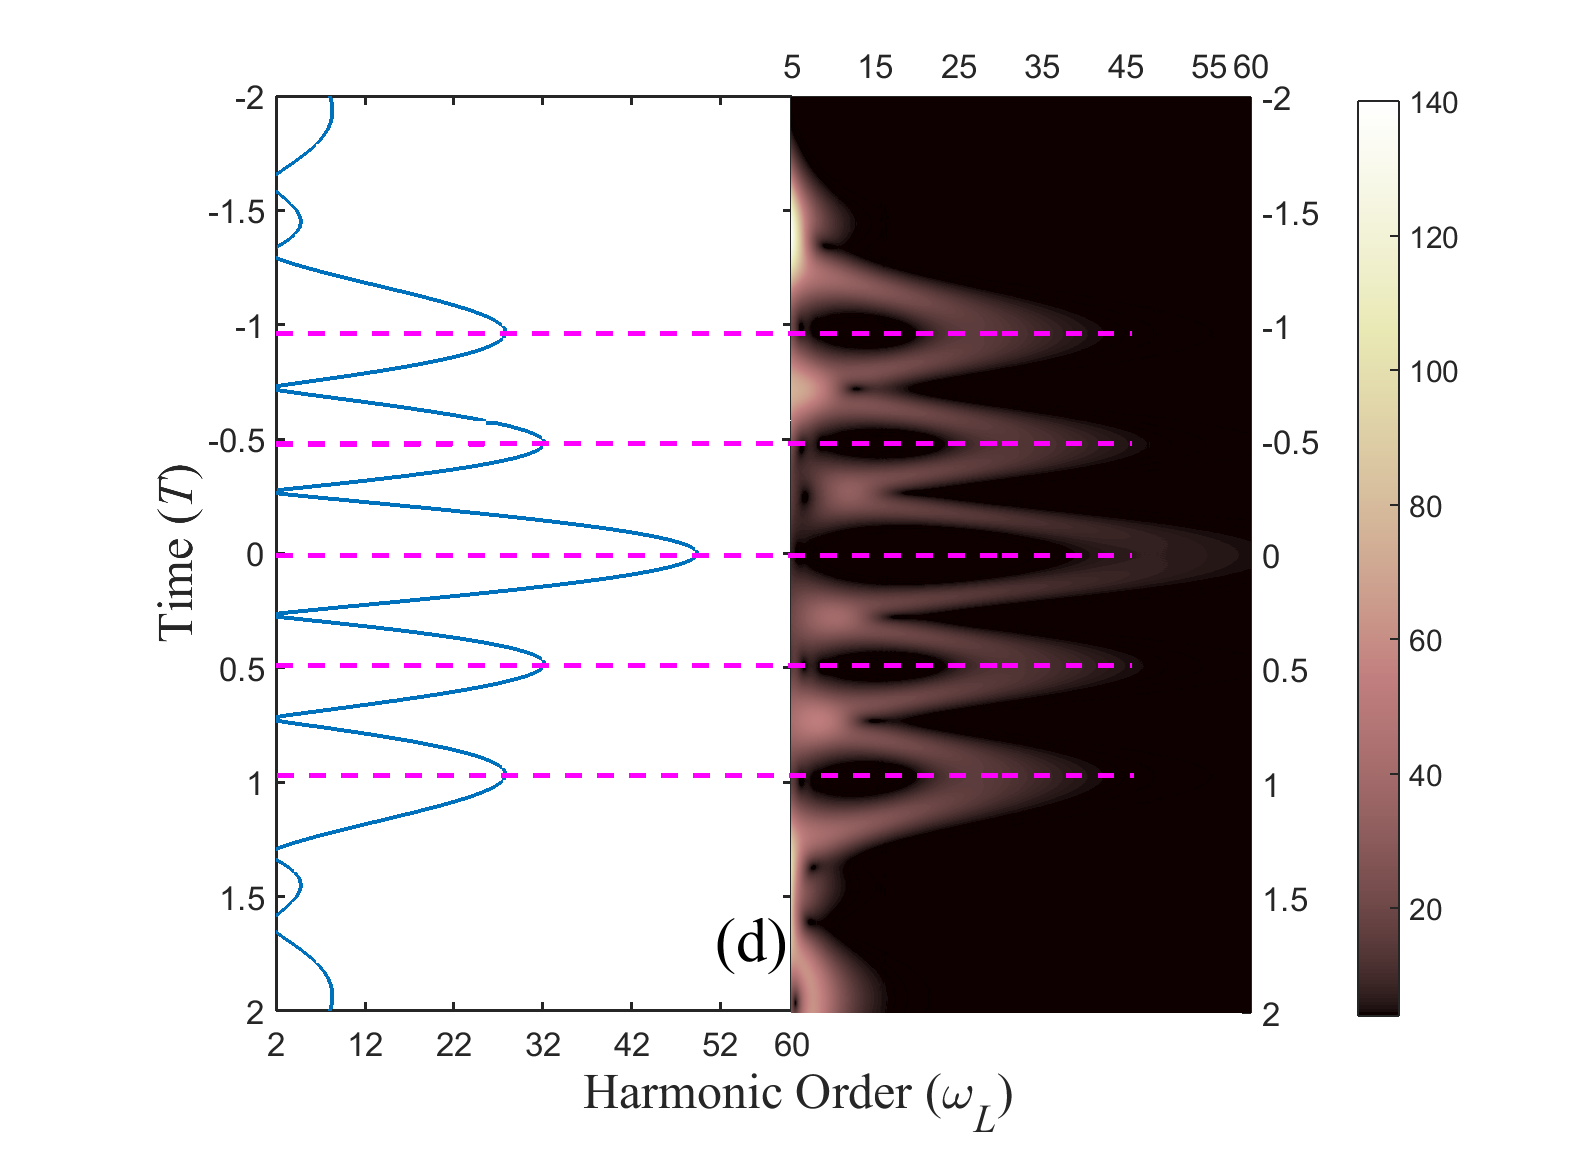
\includegraphics[width=0.45\textwidth,height=0.3\textwidth]{fig2d.eps}
	}
	\subfigure{
		\label{fig2e}
		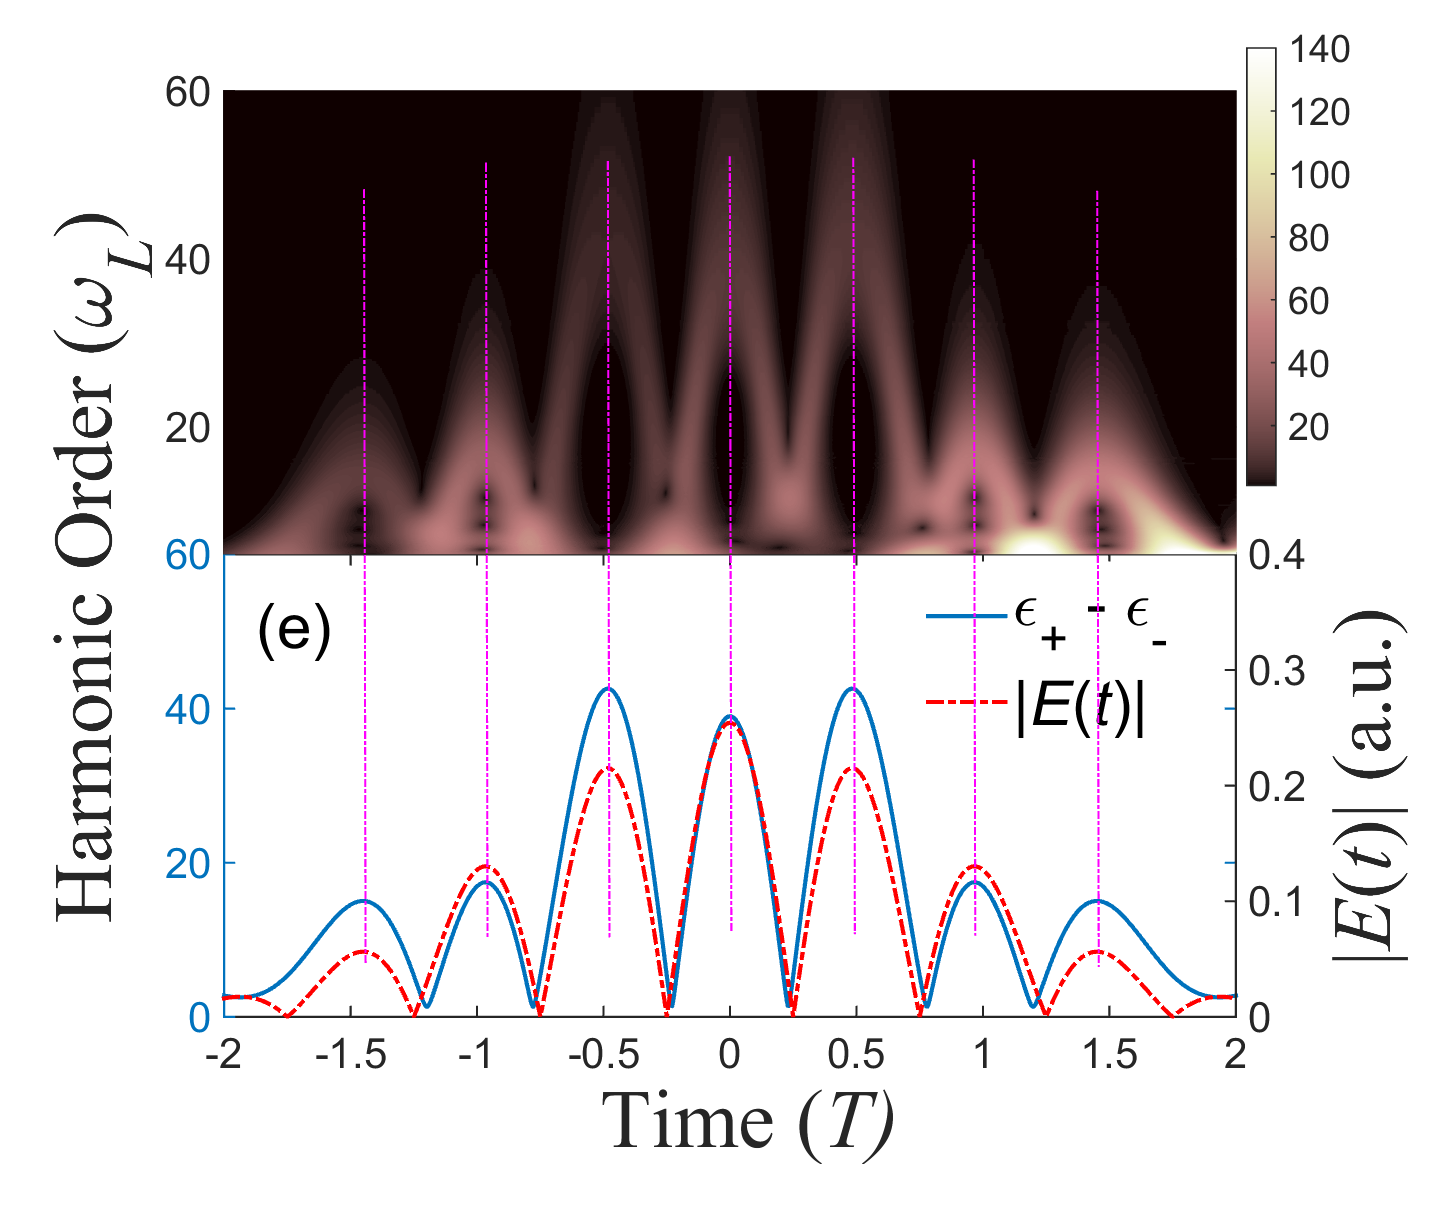
\includegraphics[width=0.42\textwidth,height=0.3\textwidth]{fig2e.eps}
	}
	\hspace{-0.05in}
	\subfigure{
		\label{fig2f}
		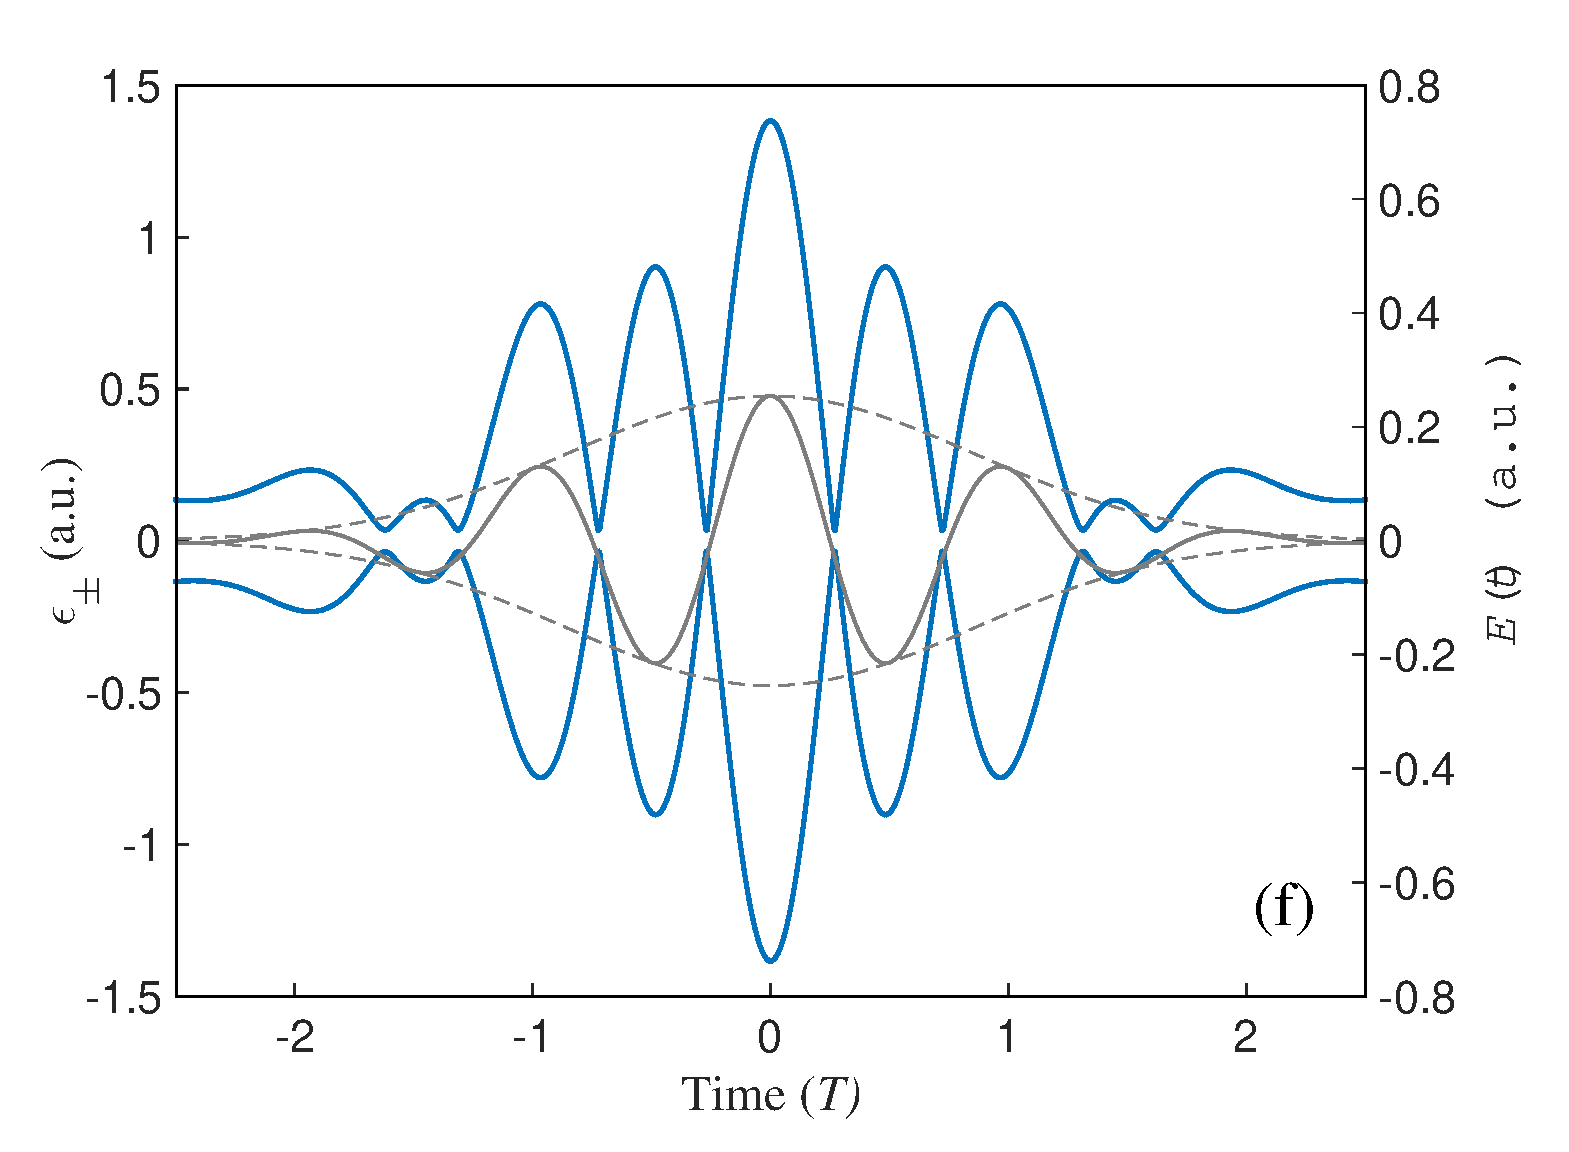
\includegraphics[width=0.42\textwidth,height=0.3\textwidth]{fig2f.eps}
	}
	\caption{HHG spectra of a laser-driven two-level system with a permanent dipole moment existing, of (a) $\mu_{11}=-4\mu_{21},\mu_{22}=4\mu_{21} (\xi=4)$, (b) $\mu_{11}=4\mu_{21},\mu_{22}=-4\mu_{21} (\xi=-4)$. (c) and (d) show their corresponding time-frequency spectra via wavelet transformations, while the left panel displays the time-dependent energy separation (unit in harmonic order) between the two dressed states. (e) and (f) show the corresponding time-dependent eigenvalue of the two dressed states. The other laser and two-level system parameters are same with those in Fig. \ref{fig1}.}
	\label{fig2}
\end{figure}
If the two-level system has no permanent dipole moment existing, that is, $\xi=0$, and the driving laser pulse is not chirped (Fig. \ref{fig1}(a)), the numerical obtained HHG spectrum is shown in Fig. \ref{fig1}(b). The spectrum possesses the generic characteristics of HHG: a plateau and a clear cutoff. The cutoff order is 11, which agree well with the predicted value $N_{\textrm{max}}$.

Now, if a permanent dipole moment is introduced, as shown in Fig. \ref{fig2}, the corresponding HHG spectrum will change significantly, even though the rest laser and two-level system parameters remain unchanged. For example, if the permanent dipole moment is $\mu_{11} =-4\mu_{21},\;\mu_{11} =4\mu_{21}(\xi=4)$ as shown in Figs. \ref{fig2a} and \ref{fig2c}, the cutoff harmonic order is extended to be about 40th, which also agree well with the prediction value $N_\textrm{max}$ by Eq. \ref{eq16}. If the permanent dipole moment is large enough [e.g., $\mu_{11} =0,\;\mu_{11} =16\mu_{21}(\xi=8)$], the harmonic plateau can  be further extended to the soft X-ray range, which would provide a possibility to synthesize a much shorter IAP or APT. It is found from the comparison of Figs. \ref{fig2c} and \ref{fig2d} that, the harmonic generation process is sensitive to the initial direction of the permanent dipole moment: for negative $\xi$ (here we call it the negative direction), the cutoff harmonic is emitted only at laser field peak time, but for positive $\xi$ (the positive direction), it is emitted at both sides of the peak with about $0.5T$ to the peak. This result can also be deduced from Eq. \ref{eq16}. In addition, Figs. \ref{fig2e} and \ref{fig2f} show the laser pulse field and time-dependent eigenvalue of two dressed states in a same figure frame for above two different permanent dipole moment cases, respectively. At the same time, with the help of Figs. \ref{fig2c} and \ref{fig2d}, it clearly demonstrates that, as Ref. \cite{CuiNi2010NJP-wavelet} says, the time-frequency spectrum shares the same shape with the laser pulse absolute amplitude. For the case of positive initial permanent dipole moment ($\xi$), there's difference existing, but it is so small that we can still consider it shares the same shape as shown in Figs. \ref{fig2c} and \ref{fig2e}.      

However, we note that and it can be seen from Figs. \ref{fig2c} and \ref{fig2d} that, the HHG spectra exhibit several well-formed individual peak structures in the plateau region, which can decrease the coherence of harmonics within this region and hence is not conducive to the IAP generation. In the following of this paper, the Gaussian pulse with a nonlinear chirped frequency is used to enhance the coherence of harmonics within the plateau region, and an attosecond pulse train with only two individual peaks can be synthesized with harmonics in the plateau region.

\begin{figure}[!htbp]
	\centering
	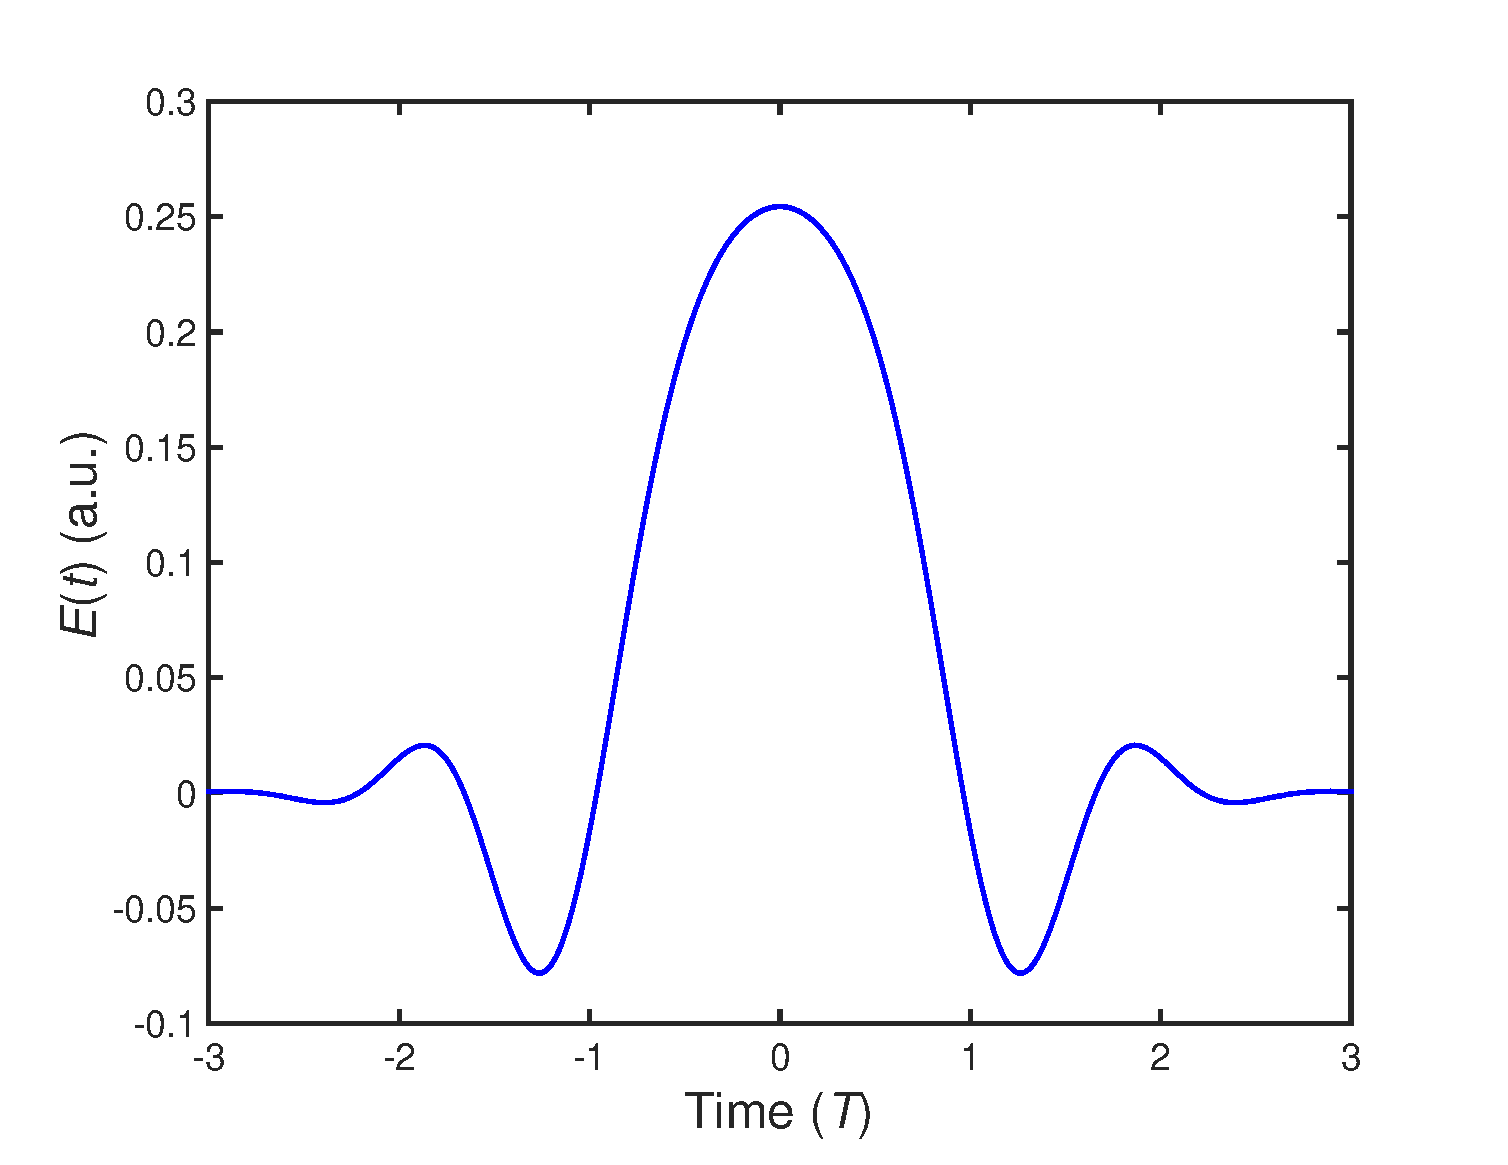
\includegraphics[width=0.45\textwidth]{fig3}
	\caption{The laser pulse with chirped frequency. $ \eta=6.25 $, $ \tau_{\rm{c}}=120 $, the other laser parameters are the same with those in Fig. \ref{fig1a}.}
	\label{fig3}
\end{figure}

The chirp chosen is with a hyperbolic tangent form \cite{Carrera-Chirp-PRA-2007}, and the time-dependent carrier envelope phase $ \varphi(t) $ in Eq. (\ref{eq3}) is then written as:

\begin{equation}
\varphi \left( t \right) =  - \eta \tanh \left[ {{{\left( {t - {t_d}} \right)} \mathord{\left/
			{\vphantom {{\left( {t - {t_d}} \right)} {{\tau _c}}}} \right.
			\kern-\nulldelimiterspace} {{\tau _c}}}} \right].
\label{eq17}
\end{equation}
Where $ \tau_{\rm{c}} $ is the steepness of the chirp function and $ t_{\rm{d}} $ is set at the middle of the sweep here. $ \eta $  denotes the frequency sweeping range. If $ \eta=0 $, driving pulse is chirp free. With a chirp, compared to the laser pulse shown in Fig. \ref{fig1a}, the temporal shape of the laser pulse changes significantly (Fig. \ref{fig3}), and its origin oscillatory periodicity and up-down symmetry disappear: the central part of the carrier wave gets broader, the side parts become weaker, while the peak amplitude is remained. Importantly, the introduce of chirp makes the absolute amplitude difference between the pulse central peak and its neighbored ones get larger. According to the rapid level crossing theory, the time-frequency HHG spectrum shares the same shape with the absolute laser pulse amplitude \cite{CuiNi2010NJP-wavelet}. Therefore, if the initial permanent dipole moment $\xi$ is negative, it's easy to speculate that HHG spectrum would have a large plateau whose harmonics just have two generation trajectories at most. This is much less than that of the case without chirp shown in Figs. \ref{fig2c} and \ref{fig2d}. Thus, these plateau harmonics obviously have better temporal coherence than that of case without chirp. However, it can be seen from Figs. \ref{fig1} and \ref{fig3} that, the introduce of chirp has weakened steepness of the laser pulse peak's rising and falling edges for the increase of time interval between the peak time and its adjacent zero time which results from the getting broader of the center carrier. We note that it is contradictory for the center carrier to get narrower and for the absolute amplitude difference between the pulse central peak and its neighbored ones to get larger, a proper group of chirp parameters are chosen as $\eta=6.25,\;\tau_{\rm{c}}=120$, which can make the absolute amplitude difference quite large and the center carrier not too broad, just as shown in Fig. \ref{fig3}.

Fig. \ref{fig4a} shows the HHG spectrum of the two-level system with a permanent dipole moment [$\mu_{11}=4,\;\mu_{22}=-4(\xi=-4)$] driven by a chirped laser pulse. With the case of Fig. \ref{fig2b} the only difference is the introduce of the chirp. The corresponding time-frequency profile of the harmonic spectrum is shown in Fig. \ref{fig4b}. Since the initial permanent dipole moment is negative, the cutoff harmonic must emit at the laser pulse peak time. In addition, the introduce of chirp doesn't change the laser pulse envelope ($E_{0}$ $\Omega_0$ remain invariant), according to Eq. \ref{eq16}, the harmonic spectra should have the same cutoff energy as the case shown in Figs. \ref{fig2b}, \ref{fig2d} and \ref{fig2f}. This is confirmed by the numerical results from Figs. \ref{fig4a} and \ref{fig4b}. There are only three well-formed individual peak structures besides the central peak in the time-frequency spectrum while the case without chirp has six because of the pulse shape changes mentioned above. Moreover, these peaks value are much smaller than those of case without chirp, this makes the value difference between the central peak and the sub-peak much larger than that of without chirp case shown in Fig. \ref{fig2d}. Therefore, within such a large plateau region, the harmonics would at most have two generation trajectories. Therefore, one can use harmonics within this region to synthesize an APT with only two individual peaks. 
\begin{figure}[!htbp]
	\centering
	\subfigure{
		\label{fig4a}
		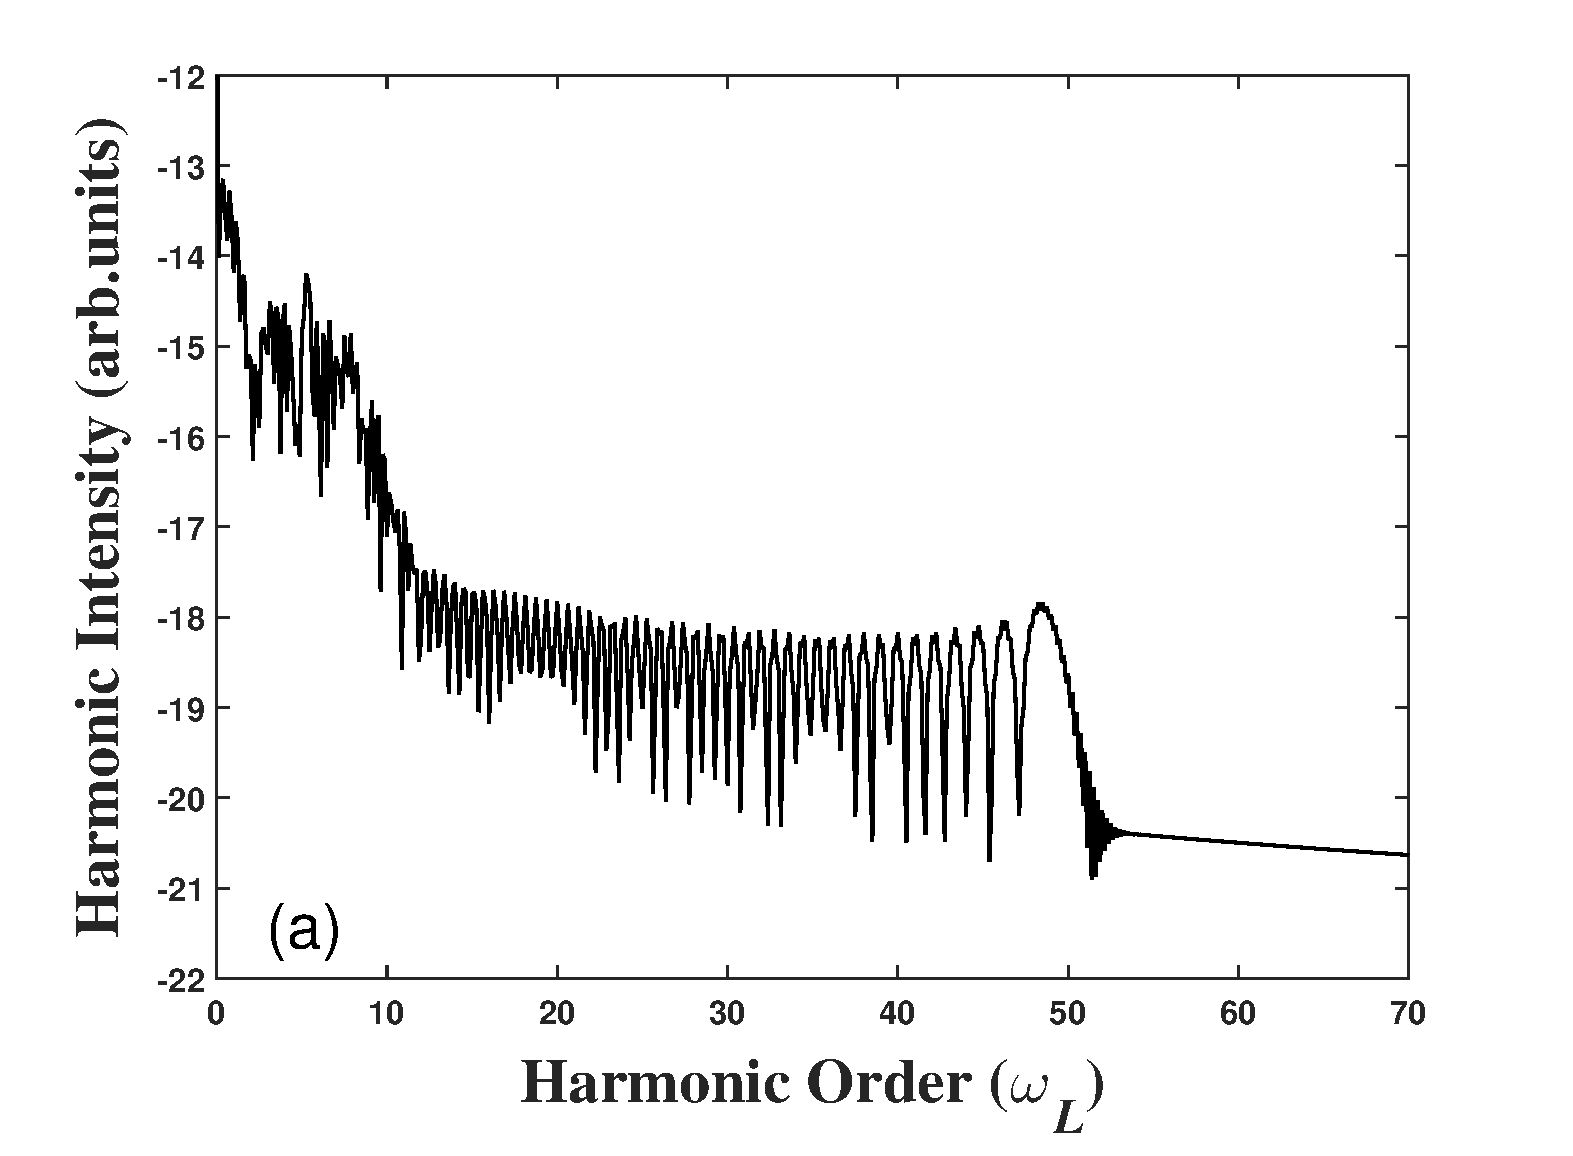
\includegraphics[width=0.40\textwidth,height=0.28\textwidth]{fig4a.eps}
	}
	\subfigure{
		\label{fig4b}
		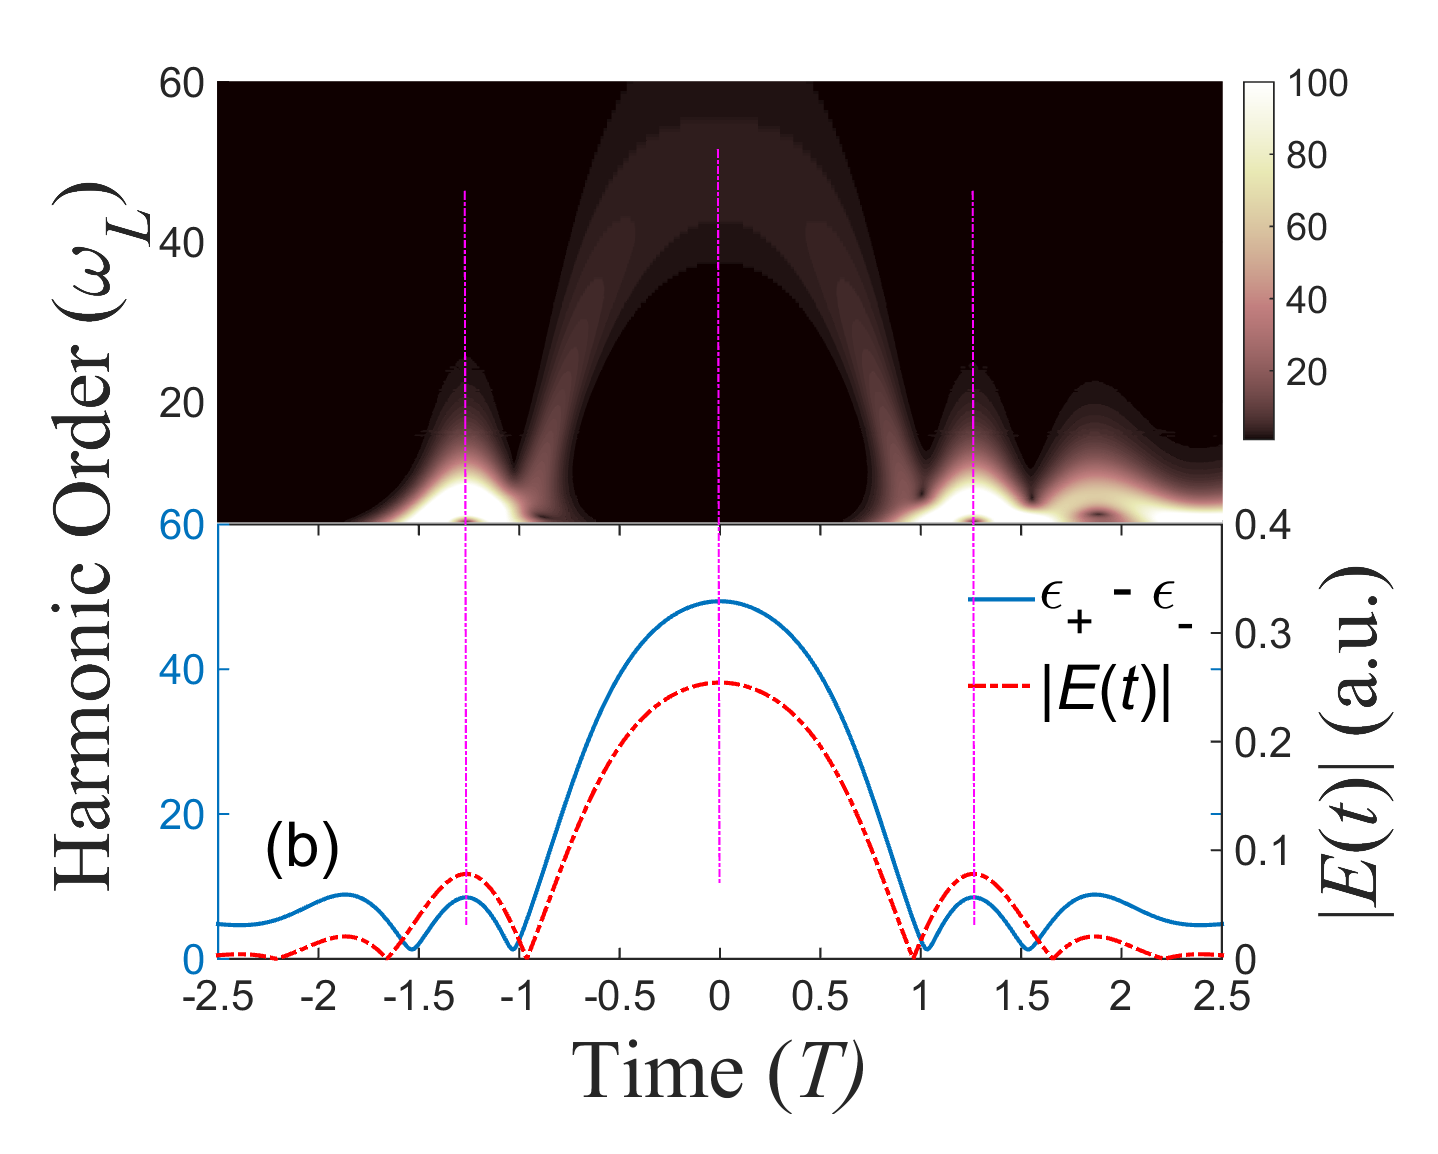
\includegraphics[width=0.45\textwidth,height=0.28\textwidth]{fig4b.eps}
	}
	\caption{(a) HHG spectrum and (b) its corresponding wavelet time-frequency analysis for a chirped-laser-driven two-level system with a permanent dipole moment [$\mu_{11}=4,\;\mu_{22}=-4(\xi=-4)$]. The left panel of figure (b) shows the time-dependent energy separation (unit in harmonic order) between the two dressed states. The other laser and two-level system parameters are same with those in Fig. \ref{fig2}.}
	\label{fig4}
\end{figure}

Next, harmonics within the plateau region generated from the system with a permanent dipole moments [$\mu_{11}=4,\;\mu_{22}=-4(\xi=-4)$]  are selected to synthesize attosecond pulses for both cases with and without chirp. All the harmonics (including the even orders) from 14th to 29th are selected for both cases. The results are shown in Figs. \ref{fig5a} and \ref{fig5b}, respectively. Every peak's FWHM is marked in the figures. There is an APT generated with ten individual peaks for the case without chirp, while there is also an APT generated which has only two individual peaks. This is completely consistent with the trajectory numbers in the plateau region (shown in Figs. \ref{fig2d} and \ref{fig4b}). Therefore, we have successfully reduced the individual peak numbers of the generated APT by introducing chirp frequency to the driving laser pulse. However, there is no IAP generated. The  increase of two center peaks' width confirms that the chirp frequency could enlarge the atto-chirp.
\begin{figure}[!htbp]
	\centering
	\subfigure{
		\label{fig5a}
		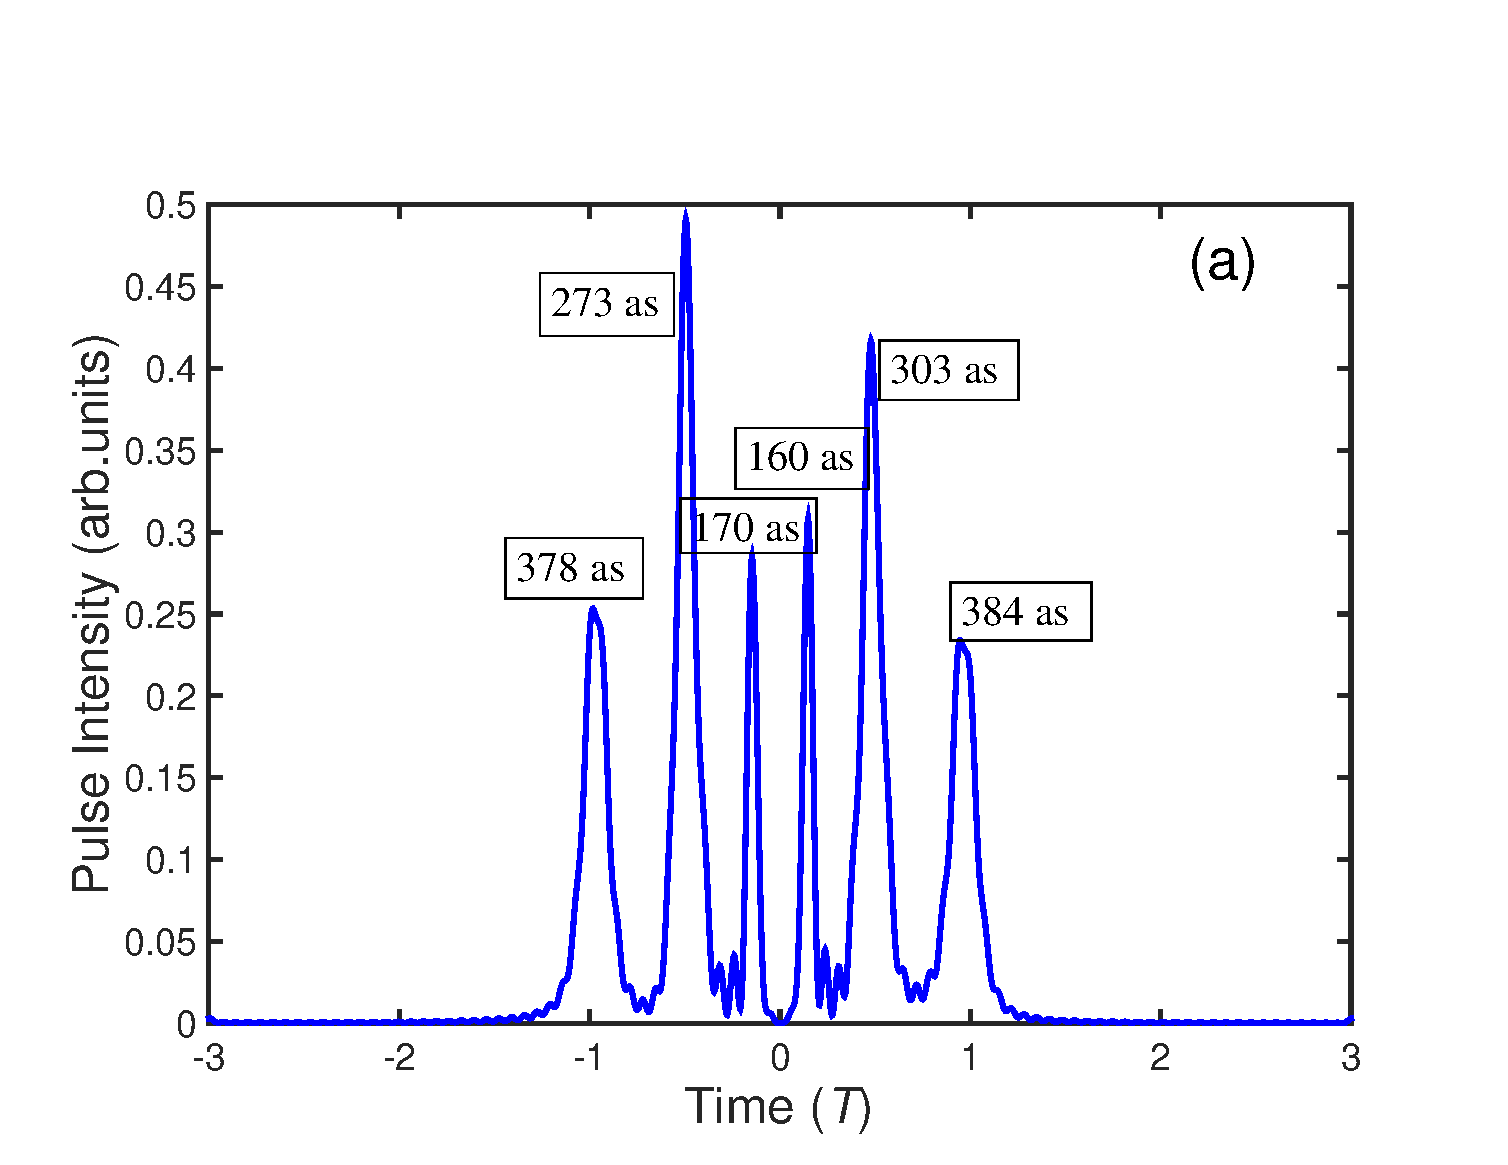
\includegraphics[width=0.4\textwidth]{fig5a.eps}
	}
%	\hspace{0.1in}
	\subfigure{
		\label{fig5b}
		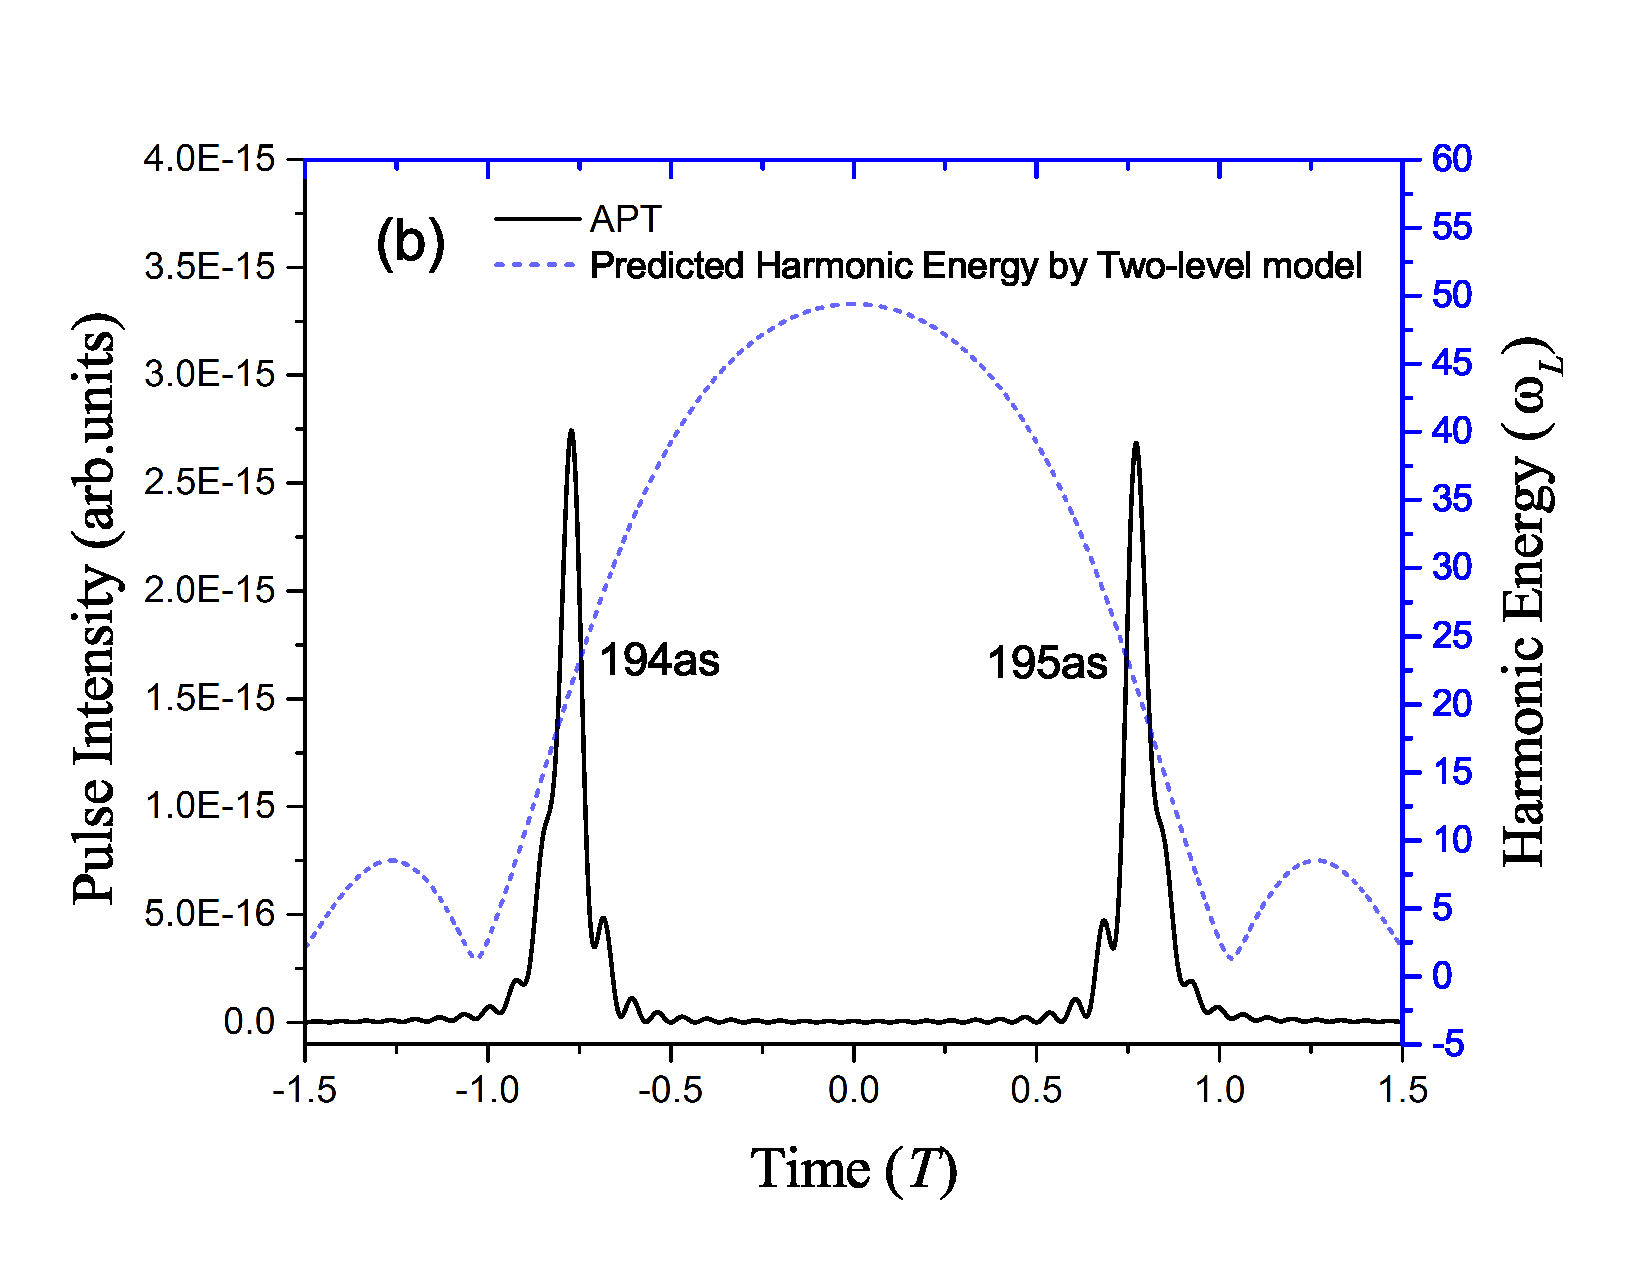
\includegraphics[width=0.4\textwidth]{fig5b.eps}
	}
	\caption{Generated attosecond pulse train (APT) by synthesizing plateau harmonics (from 14th to 29th) driven by a laser pulse (a) without chirp and (b) with chirp. The other laser and two-level system parameters are same with those in Fig. \ref{fig4}. The blue dashed curve is the harmonic energy predicted by the two-level model same with Figs. \ref{fig2c} and \ref{fig2d}.}
	\label{fig5}
\end{figure}
	
Thus we have demonstrated that the combination of controls, introduce of permanent dipole moment to two-level system and chirp frequency to driving laser pulse, has big influences on the HHG and attosecond pulse generation process. Due to the permanent dipole moment, much more plateau harmonics are generated and used to synthesize a shorter attosecond pulse; on the other hand, the chirp frequency could reduce the generation trajectory numbers of plateau harmonics to a minimum of two which can finally lead to an APT generated with only two individual peaks. However, the pulse intensity is much weaker than that of the case without chirp (Fig. \ref{fig5}). In view of this, a method that could enhance the harmonic signal intensity should be proposed to make up the intensity loss for introducing the chirp frequency. Here, we will investigate the propagation conditions and expect it can enhance the harmonic intensity. One part medium parameters are chosen as: , $ T_{1}=1.0\times10^{-12} \textrm{s} $, $ T_{2}=0.5\times10^{-12} \textrm{s} $ \cite{Kalosha-Two-Level-PRL-1999} and the rest medium and all the laser parameters are all the same with those of non-propagation cases in Fig. \ref{fig5}. Initial condition of the laser pulse was given in part \emph{theoretical models and methods}. As for the chirped laser pulse, the initial condition is
\begin{equation}
\begin{array}{l}
{E_x}\left( {z,t = 0} \right) = {E_0}\exp \left[ { - 4\ln 2{{\left( {\frac{{z - {z_0}}}{{c\tau }}} \right)}^2}} \right]\cos \left[ {{\omega _L}{{\left( {z - {z_0}} \right)} \mathord{\left/
			{\vphantom {{\left( {z - {z_0}} \right)} c}} \right.
			\kern-\nulldelimiterspace} c} + \eta \tanh \frac{{z - {z_0}}}{{c{\tau _c}}}} \right],\\
{H_y}\left( {z,t = 0} \right) = \sqrt {{{{\varepsilon _0}} \mathord{\left/
			{\vphantom {{{\varepsilon _0}} {{\mu _0}}}} \right.
			\kern-\nulldelimiterspace} {{\mu _0}}}} {E_x}\left( {z,t = 0} \right).
\end{array}
\label{eq20}
\end{equation}

\begin{figure}[!htbp]
\centering
	\subfigure{
		\label{fig6a}
		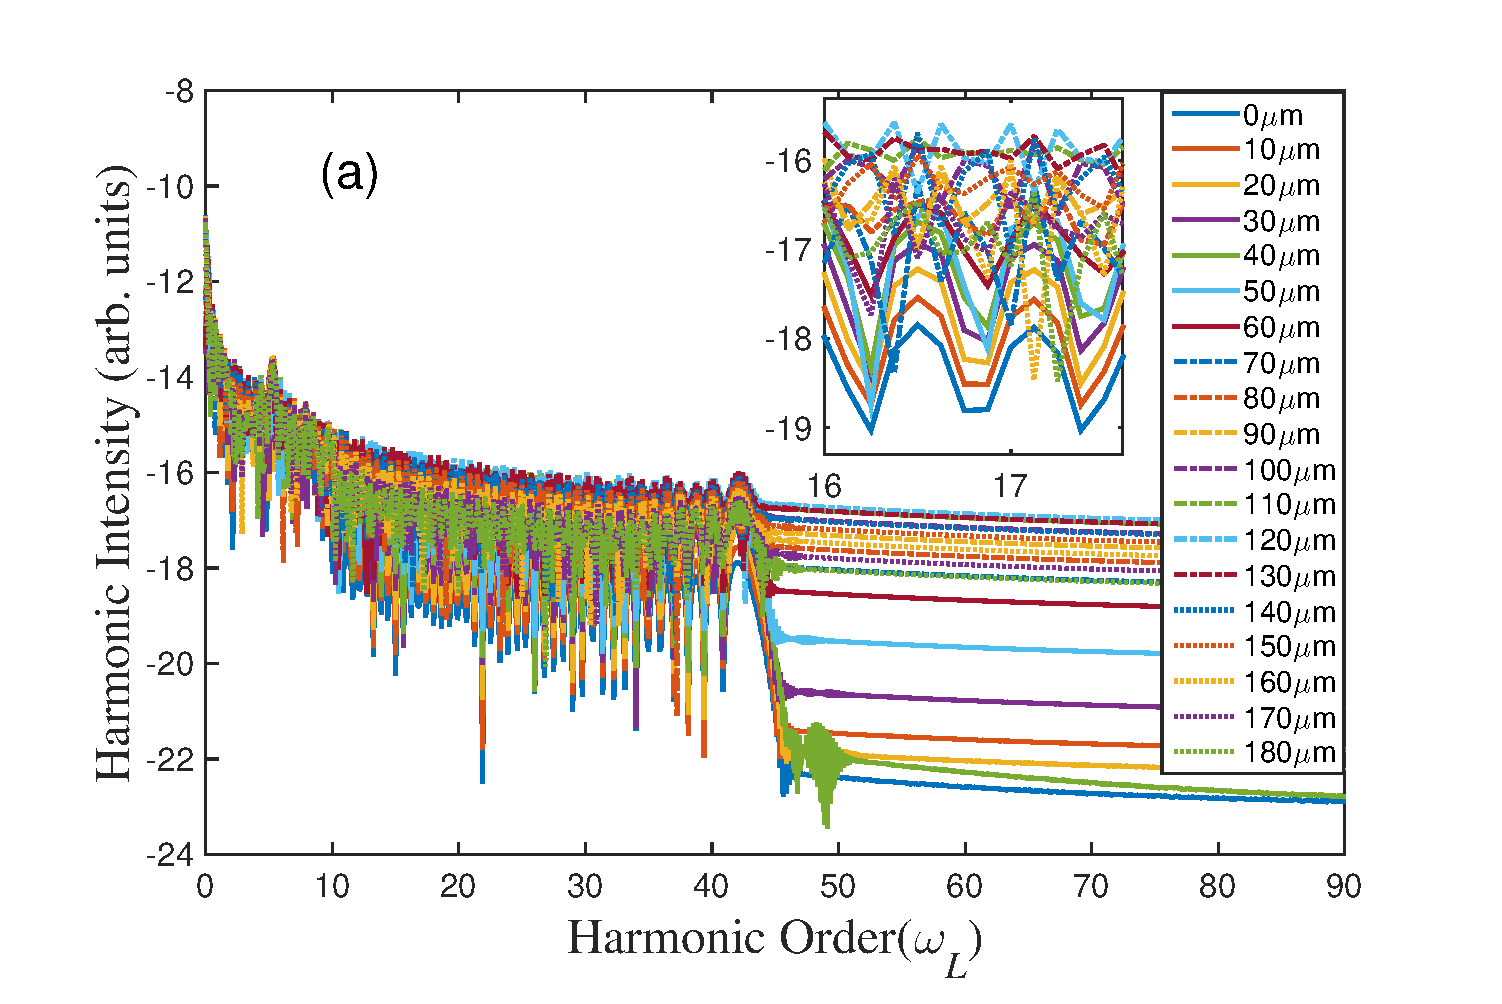
\includegraphics[width=0.45\textwidth]{fig6a.eps}
	}
	\hspace{-0.3in}
	\subfigure{
		\label{fig6b}
		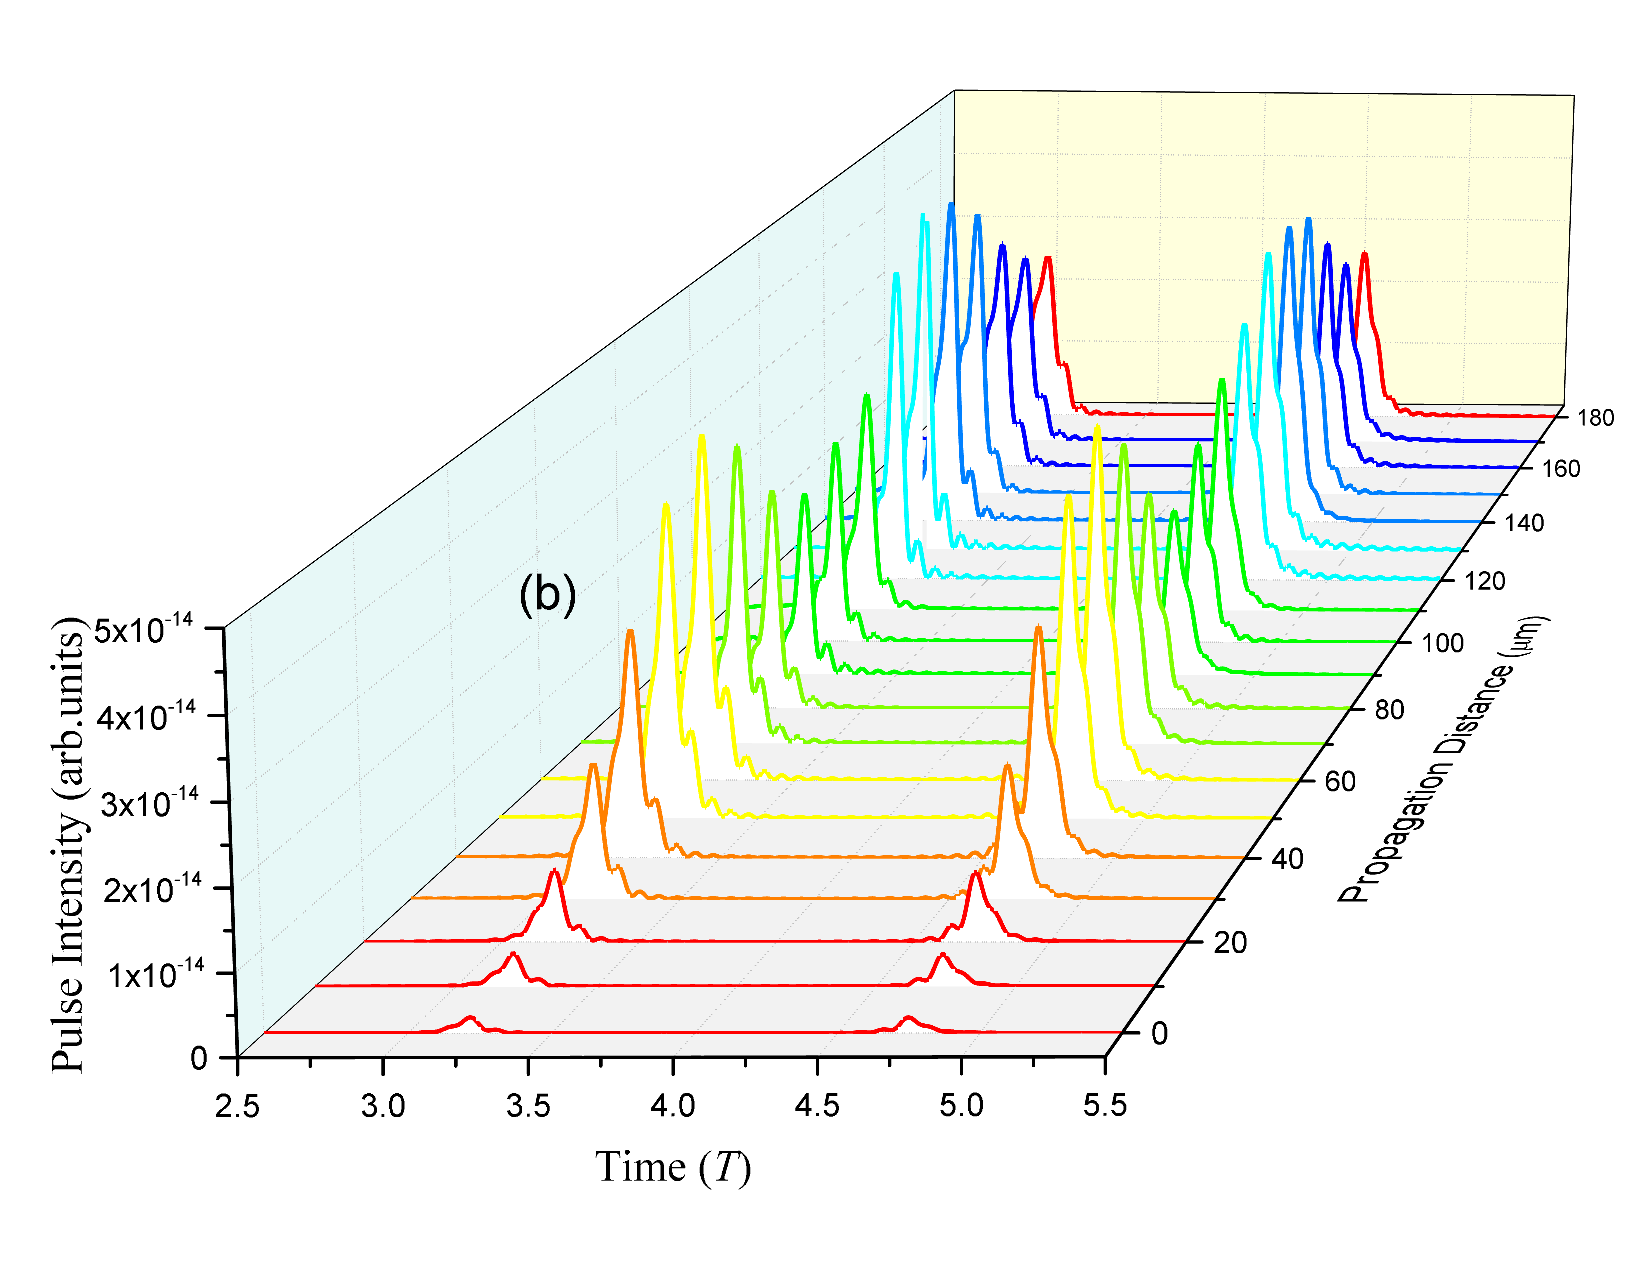
\includegraphics[width=0.45\textwidth]{fig6b.eps}
	}
	\subfigure{
		\label{fig6c}
		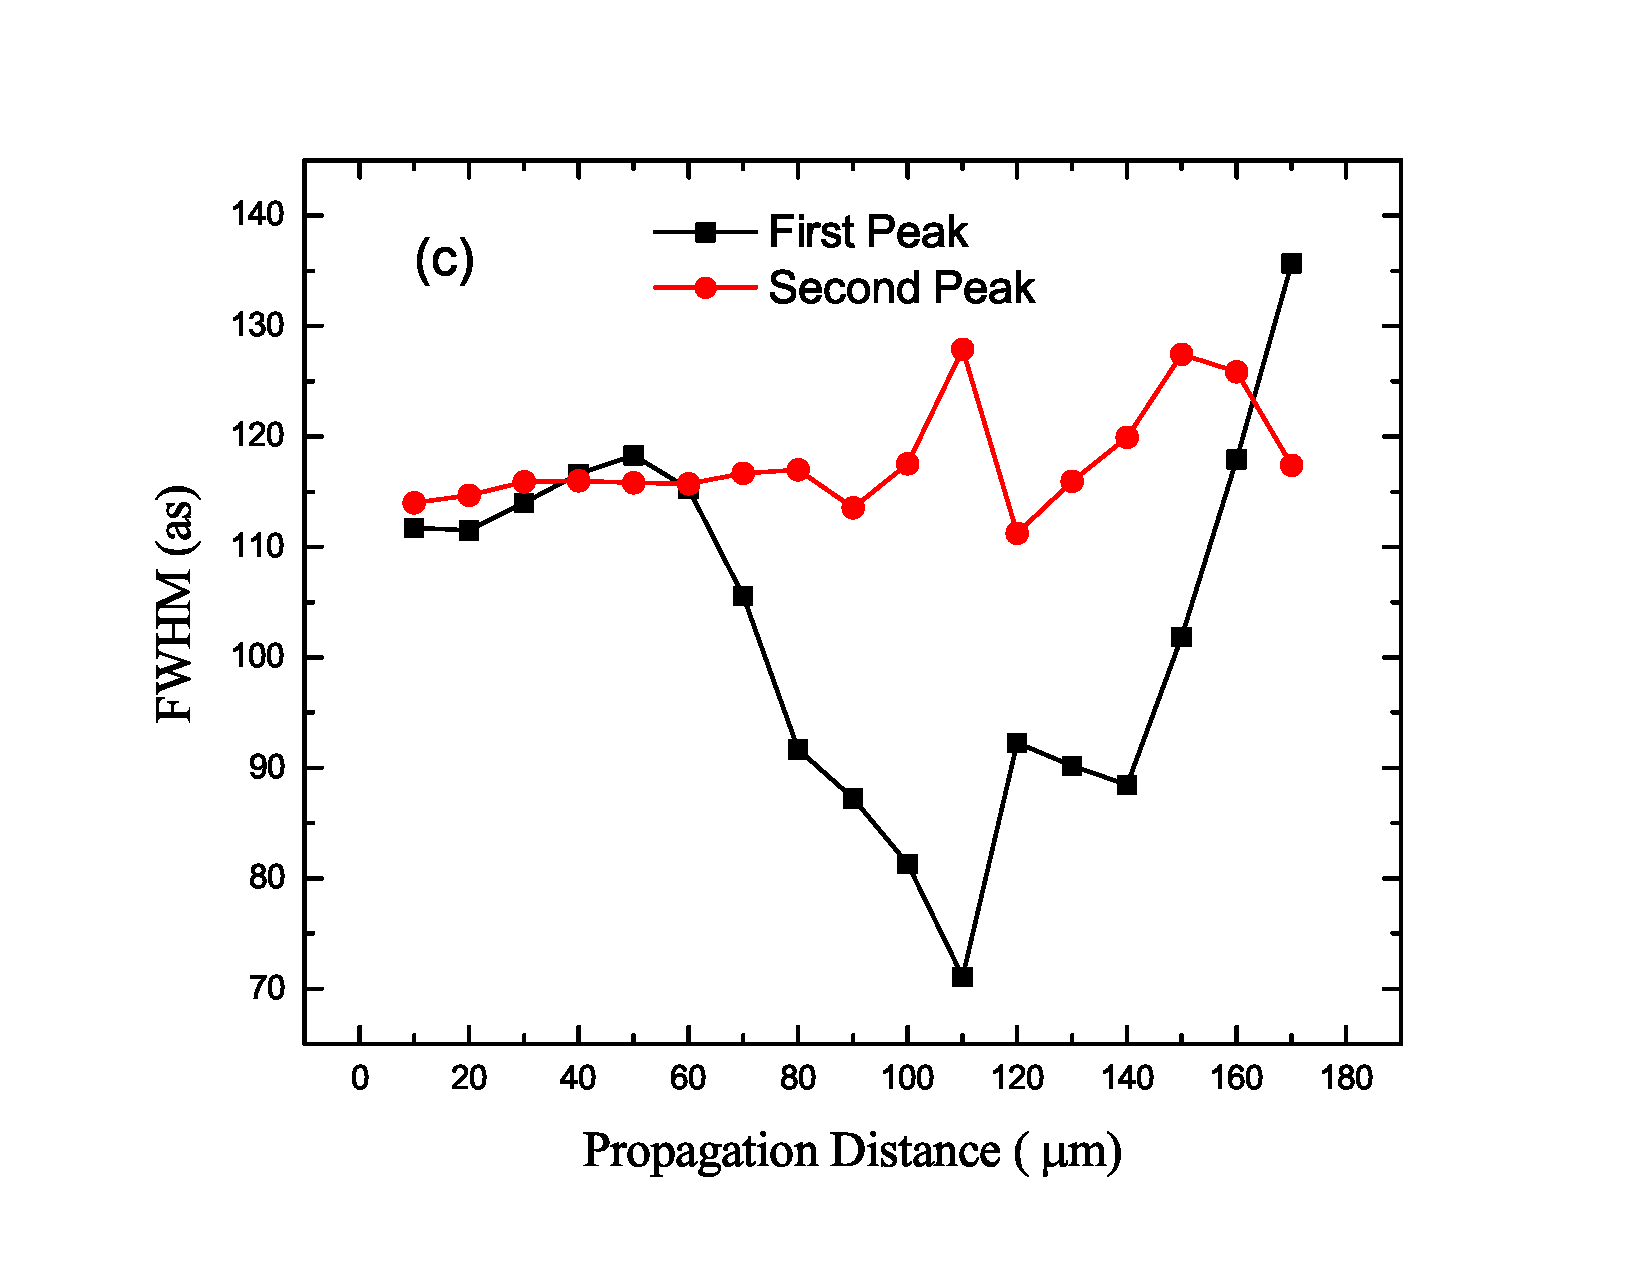
\includegraphics[width=0.5\textwidth]{fig6c.eps}
		}
\caption{(a) Seventeen groups of harmonic spectra corresponding to seventeen groups of propagation distance. (b) Generated APTs by synthesizing plateau harmonics (between 14th to 29th) of spectra (a). (c) The FWHMs of generated APTs. Two-level system has a permanent dipole moment of $\mu_{11}=4,\;\mu_{22}=-4(\xi=-4)$. The laser pulse and other two-level system parameters are same with those of Fig. \ref{fig5}.}
\label{fig6}
\end{figure}

Seventeen groups of propagation distance are investigated from 10 to 170 $ \mu $m evenly divided by 10 $ \mu $m, the harmonic generation in the transmission interface will be studied, respectively.
The simulation results are shown in Fig. \ref{fig6}. A peak appears in the position of about  $ 5.36\;\omega_{\rm{L}} $ with considerable value. We know that it is the results of the resonant absorption, and this peak also exists in the non-propagation case but it is not so strong. Here we will focus on the cutoff region of the spectrum because we can only synthesize the continuum harmonics within this region to generate an IAP. It shows that, for the both cases, the harmonic intensity varies with different propagation distance. However, this variation is not monotonically increasing or monotonically decreasing. There is a maximum value with the propagation of the laser pulse. We select $37\rm{th}$-$50\rm{th}$ and $41\rm{st}$-$45\rm{th}$ harmonics in the cutoff region for the chirp case and the non-chirp case, respectively, to synthesize an IAP. Fig. \ref{fig7} shows the results and Table \ref{table1} is the corresponding statistics for the generated pulse peak intensity and the FWHM. Even though the selected harmonics are in the cutoff region, the synthesized IAP can be as strong as those pulses synthesized by selecting the plateau harmonics [Fig. \ref{fig5a}] and even stronger than the two generated pulses of the chirp case [Fig. \ref{fig5b}]. However, the pulse intensity cannot progressively increase, it will has a maximum value for an proper propagation distance. And the pulse for the chirp or non-chirp case almost has the same duration for different propagation distance because of the same harmonics selected. We note that, for the modulation of the chirped frequency, the spectral width of the continuum is different for the two cases. We will select harmonics as much as possible to synthesize more intensive IAP. Therefore we selected different orders of harmonic for the two cases, while this cannot influence our demonstration  since only the propagation effect is studied here.

We can also see from Fig. \ref{fig7} and Table \ref{table1} that, the chirped frequency has no help with the IAP generation because of the selecting of cutoff region harmonics instead of plateau region harmonics. Furthermore, even though the propagation can increase the intensity of cutoff region harmonics, it has hardly increased the plateau harmonics (seen from Fig. \ref{fig6}). Therefore, if we want to generate an IAP, the propagation is helpful. Otherwise, the propagation is not needed, and the medium should be low-density or thin enough.

%\begin{table}[!htbp]
%	\centering
%	\caption{Statistics for the isolated attosecond pulse's peak intensity and FWHM for the two cases of with and without chirp.}
%\begin{tabular}{cccccc}
%	\hline
%	Propagation & \multicolumn{2}{c}{Laser pulse without chirp} &  & \multicolumn{2}{c}{Laser pulse with chirp}\tabularnewline
%	\cline{2-3} \cline{5-6}
%	distance ($\mu m$) & Peak intensity (arb.units) & FWHM (as) &  & Peak intensity (arb.units) & FWHM (as)\tabularnewline
%	\hline
%	10 & 0.32 & 325 && 0.03 & 950\tabularnewline
%	20 & 0.25 & 325 && 0.03 & 950\tabularnewline
%	30 & 0.19 & 300 && 0.06 & 980\tabularnewline
%	40 & 0.14 & 300 && 0.11 & 950\tabularnewline
%	50 & 0.13 & 300 && 0.22 & 950\tabularnewline
%	60 & 0.23 & 300 && 0.36 & 980\tabularnewline
%	70 & 0.46 & 300 && 0.48 & 950\tabularnewline
%	80 & 0.48 & 300 && 0.51 & 950\tabularnewline
%	90 & 0.09 & 300 && 0.44 & 950\tabularnewline
%	\hline
%\end{tabular}
%	\label{table1}

%\end{table}

\section{Conclusions}
In this paper, we tried to combine the control of the matter and the control of the driven laser pulse to produce a high-order harmonic spectrum with a higher cutoff energy and strong coherence. It is shown that the existence of the permanent dipole moments can significantly extend the plateau of the harmonic spectrum. If the laser pulse is modulated by added chirped frequency, the up-down symmetry of the laser field will be dramatically changed. This kind of laser pulse can exactly enhance the coherence of the harmonics in a large range in the plateau of the high-order harmonic spectrum. Finally, an attosecond pulse train with only two individual peaks is generated by Fourier synthesis of the harmonics within the plateau region. If the propagation effect is considered, an isolated attosecond pulse with considerable intensity can be generated by synthesizing the harmonics in the spectrum cutoff region for a proper propagation distance.

\section*{Acknowledgments}
This work is supported by the National Natural Science Foundation of China (NNSF, Grant
No.11374318). C.L. appreciates the supports from the 100-Talents Project of Chinese Academy
of Sciences and Department of Human Resources and Social Security of China.

\end{document}

